% \setcounter{section}{0}%更改chapter的计数器值
% %\numberwithin{equation}{chapter}%公式计数器从属于节计数器
% \numberwithin{equation}{section}%公式计数器从属于节计数器
% \numberwithin{figure}{section}%图计数器从属于节计数器
% \setcounter{chapter}{8}

%\chapter{\texorpdfstring{高阶振幅}{9 Higher order amplitudes}}
\chapter{高阶振幅} \label{cha:9}
在本章我们将讨论弦论的高阶振幅. 前半段的主要目标是理解弦微扰论的有限性与幺正性. 在细致地讨论树图振幅之后,我们会考察一般振幅. 利用因子化的思想将高阶振幅与低阶振幅相关联之后,我们将讨论一些致力于理解所有阶乃至非微扰弦论的思想.

%\section{\texorpdfstring{一般的树图振幅}{9.1 General tree-level amplitudes}}
\section{一般的树图振幅}
第6章初步考察了某些简化树图振幅的计算. 用一个树图振幅的一般分析展开本章将是有益的,它将会阐明一些会在高阶振幅出现的模块. 我们将专注于定向闭弦,以及三点振幅和四点振幅,它们会阐明一些重要特征. 主要议题是收敛与“幺正性”. 后一项含义比较宽泛. 既指S矩阵的幺正性$S S^{\dagger}=1$, 又指Hilbert空间的正定性. 当然,我们从第4章已经获知BRST上同调有一个正定内积,这使得我们需要证明的是振幅会遵循BRST不变性:唯一的BRST态是可产生的,并且BRST等价态的振幅是相等的. 对于后者,我们在5.4节给出了一般讨论,但在这里可以更加清晰地阐释.\\
在进入一般分析之前,我们先来回忆一些对计算有用的结果. 假定我们有 $d$个无限平坦维,快子顶点算符归一化成
\begin{equation}
	g_{\mathrm{c}, d}: e^{i k \cdot X}:
\end{equation}
例如,在一个维度环向紧致化的情况中,我们有$g_{\mathrm{c}, 25}=g_{\mathrm{c}}(2 \pi R)^{-1 / 2}$ .  那么,对于一般OCQ顶点算符的物质部分,正确的归一化可由OPE中最奇异的一项固定
\begin{equation}
	\mathscr{V}_{j}(k ; z, \bar{z}) \overline{\mathscr{Y}_{j^{\prime}}(k ; 0,0)}=\frac{g_{\mathrm{c}, d}^{2}}{z^{2} \bar{z}^{2}}+\ldots
\end{equation}
其中bar代表Euclidean 共轭 (6.7.28). 由于顶点算符权重为(1,1),奇点是 $|z|^{-4}$,重复快子极点计算 (6.6.7) 就给出归一化
\begin{equation}
	\begin{aligned}
		&e^{-2 \lambda}\left\langle\tilde{c}\left(\bar{z}_{1}\right) c\left(z_{1}\right) \tilde{c}\left(\bar{z}_{2}\right) c\left(z_{2}\right) \tilde{c}\left(\bar{z}_{3}\right) c\left(z_{3}\right): e^{i k \cdot X}(z, \bar{z}):\right\rangle \\
		=&\frac{8 \pi i}{\alpha^{\prime} g_{c, d}^{2}}\left|z_{12} z_{13} z_{23}\right|^{2}(2 \pi)^{d} \delta^{d}(k)
	\end{aligned}
\end{equation}
所有S矩阵中的所有归一化常数都写成 $g_{\mathrm{c}, d}=\kappa_{d} / 2 \pi$.

\subsection*{\centerline{Three-point amplitudes(三点振幅)}}
我们首先将树图振幅表示成几个有用的形式. 对于一般的树图三点振幅,弦S矩阵的规范固定表达式 (5.3.9) 约化至三个固定顶点算符的路径积分
\begin{equation}
	S_{S_{2}}(1 ; 2 ; 3)=e^{-2 \lambda}\left\langle\hat{\mathscr{V}}_{1}^{\prime}(\infty, \infty) \hat{\mathscr{V}}_{2}(1,1) \hat{\mathscr{V}}_{3}(0,0)\right\rangle_{S_{2}}
\end{equation}
其中的数字' $n$ '是弦动量和态$(k_n, j_n)$的缩写. hat指明顶点算符处在固定绘景中————即,对位置的积分不引入鬼场插入. 正如我们在5.4节中讨论的,这一形式自然地来自于态-算符对应, 并在OCQ情况中取如下的形式
\begin{equation}
	\hat{\mathcal{V}}_{j}=\tilde{c} c \mathscr{V}_{j}
\end{equation}
利用6.7节中的结果,可将球面上的路径积分转化成矩阵元,这个振幅也可表示成矩阵元或算符乘积系数:
\begin{equation}
	S_{S_{2}}(1 ; 2 ; 3)=e^{-2 \lambda}\left\langle\hat{\mathcal{Y}}_{1}\left|\hat{\hat{V}}_{2}(1,1)\right| \hat{\hat{V}}_{3}\right\rangle=e^{-2 \lambda} c_{123}
\end{equation}
这将时空中的振幅与世界面上的矩阵元关联起来,并进一步与编码(encode)CFT定域性质的算符乘积系数相联系. \\
第一个议题是BRST-null态的退耦,这使得BRST-等价态有相同的振幅. 假定三点振幅中的 $\left|\hat{\mathscr{V}}_{3}\right\rangle$ 是 null态
\begin{equation}
	\left|\hat{\mathscr{V}}_{3}\right\rangle=Q_{\mathrm{B}}|\chi\rangle
\end{equation}
那么
\begin{equation}
	\begin{aligned}
		e^{2 \lambda} S_{S_{2}}(1 ; 2 ; 3) &=\left\langle\hat{\mathscr{V}}_{1}\left|\left[\hat{\mathscr{V}}_{2}(1,1), Q_{\mathrm{B}}\right]\right| \chi\right\rangle+\left\langle\hat{\hat{\jmath}}_{1}\left|Q_{\mathrm{B}} \hat{\mathscr{V}}_{2}(1,1)\right| \chi\right\rangle \\
		&=0
	\end{aligned}
\end{equation}
由于态2和1的BRST不变性,所以它们分别为零. 类似地,如果 $\hat{\mathscr{V}}_{2}=\left\{Q_{\mathrm{B}}, \chi\right\}$ 或 $\left|\hat{\mathscr{V}}_{1}\right\rangle=Q_{\mathrm{B}}|\chi\rangle$ ,振幅也为零. 我们必须在这里使用Hilbert空间形式理论,但值得用路径积分的语言重复相同的讨论. 假定 $\mathscr{V}_{3}$ 是null
\begin{equation}
	\hat{\mathcal{V}}_{3}=Q_{\mathrm{B}} \cdot \mathscr{X}
\end{equation}
将球面上的围道积分扩展,使之远离 $\mathscr{X}$ ,直到它变成绕 $\hat{\mathscr{V}}_{1}$ 的小圈加上绕 $\hat{\mathscr{V}}_{2}$的小圈. 它们由于BRST不变为零, $Q_{\mathrm{B}} \cdot \hat{\mathscr{V}}_{1}=Q_{\mathrm{B}} \cdot \hat{\mathscr{V}}_{2}=0$.\\
那么到这一阶,振幅在物理Hilbert空间是定义好的. 即BRST上同调. 与时空坐标不变性相对应的null引力子的退耦,是BRST-null退耦的特殊情况. 那么自然会有这样的问题,时空坐标不变性是否是某个更大对称性的一部分?我们会在9.6节回到这个问题. \\
我们现在考察S矩阵的幺正性
\begin{equation}
	\sum_{n} S_{m n} S_{p n}^{*} \stackrel{?}{=} \delta_{m p}
\end{equation}
这等价于几率守恒. 将S矩阵拆成常数项与散射项
\begin{equation}
	S_{m n}=\delta_{m n}+i T_{m n}
\end{equation}
那么对于散射矩阵 $T$, 幺正性暗示了
\begin{equation}
	T_{m p}-T_{p m}^{*}=i \sum_{n} T_{m n} T_{p n}^{*}
\end{equation}
根据定义,T矩阵至少包括三个粒子,所以对于球面上的三粒子振幅, (9.1.12)的右边为零. 那么幺正性给出
\begin{equation}
	T_{S_{2}}(1 ; 2 ; 3)=T_{S_{2}}(-1 ;-2 ;-3)^{*}
\end{equation}
其中负号代表将入顶点算符换成出顶点算符. 如果入顶点算符与出顶点算符之间的关系是
\begin{equation}
	\hat{\mathscr{V}}_{-i}=-\overline{\hat{\nu}_{i}}
\end{equation}
那么 (9.1.13) 就是满足的.\\
这是一个自然的定义:共轭将 $e^{i k \cdot X}$变成 $e^{-i k \cdot X}$, 出射变入射,对于其他量子数类似. 引入负号是为了抵消$\tilde{c} c$ 顺序的调换,这使得 $\hat{\mathscr{V}}_{-i}$ 仅是对顶点算符所有显含i的因子取共轭. 那么路径积分的共轭给出
\begin{equation}
	\left\langle\hat{\mathscr{V}}_{1}^{\prime}(\infty, \infty) \hat{\mathscr{V}}_{2}(1,1) \hat{\mathscr{V}}_{3}(0,0)\right\rangle_{S_{2}}=-\left\langle\hat{\mathscr{V}}_{-1}^{\prime}(\infty, \infty) \hat{\mathscr{V}}-2(1,1) \hat{\mathscr{V}}-3(0,0)\right\rangle_{S_{2}}^{*}
\end{equation}
这暗示了幺正关系 (9.1.13). 想当然的看,这个路径积分显然是实的,(9.1.15)中不应有负号. 但是,我们记起这个路径积分必须通过特定的解析延拓定义,而显式结果(6.2.6) 因此获得总因子$i$ .

\subsection*{\centerline{Four-point amplitudes and world-sheet duality(四点振幅和世界面对偶)}}
连通四点振幅是
\begin{equation}
	S_{S_{2}}(1 ; 2 ; 3 ; 4)=e^{-2 \lambda} \int_{\mathbf{C}} d^{2} z\left\langle\hat{\mathscr{V}}_{1}^{\prime}(\infty, \infty) \hat{\mathscr{V}}_{2}(1,1) \hat{\mathscr{V}}_{3}(0,0) \mathscr{V}_{4}(z, \bar{z})\right\rangle_{S_{2}}
\end{equation}
将这一期望值写成一个矩阵元给出
\begin{equation}
	\left\langle\hat{\mathscr{V}}_{1}\left|\mathrm{~T}\left[\hat{\mathscr{V}}_{2}(1,1) \mathscr{V}_{4}(z, \bar{z})\right]\right| \hat{\mathscr{V}}_{3}\right\rangle
\end{equation}
对于OCQ顶点算符,鬼场期望值是常数. 但为了与普遍情况相联系,将这个鬼场稍微移动一点更有用. 利用围道讨论,对 $d^{2} z$ 积分的鬼场插入可以写成
\begin{equation}
	\mathscr{V}_{4}(z, \bar{z})=(z \bar{z})^{-1}\left\{b_{0},\left[\tilde{b}_{0}, \hat{\mathscr{V}}_{4}(z, \bar{z})\right]\right\}
\end{equation}
利用上式以及  $b_{0}$与 $\tilde{b}_{0}$湮灭物理态的条件 (4.3.29) ,矩阵元变成
\begin{equation}
\begin{aligned}
&\theta(1-|z|)\left\langle\hat{\mathscr{V}}_{1}\left|\hat{\mathscr{V}}_{2}(1,1) b_{0} \tilde{b}_{0} z^{L_{0}-1} \bar{z}^{\tilde{L}_{0}-1} \hat{\mathscr{V}}_{4}(1,1)\right| \hat{\mathscr{V}}_{3}\right\rangle \\
+&\theta(|z|-1)\left\langle\hat{\mathscr{V}}_{1}\left|\hat{\mathscr{V}}_{4}(1,1) b_{0} \tilde{b}_{0} z^{-L_{0}-1} \bar{z}^{-\tilde{L}_{0}-1} \hat{\mathscr{V}}_{2}(1,1)\right| \hat{\mathscr{V}}_{3}\right\rangle
\end{aligned}
\end{equation}

我们在矩阵元中插入中间态的完备基
\begin{equation}
	\begin{aligned}
		&\theta(1-|z|) \sum_{i, i^{\prime}} z^{\alpha^{\prime}\left(k_{i}^{2}+m_{i}^{2}\right) / 4-1} \bar{z}^{\alpha^{\prime}\left(k_{i}^{2}+\tilde{m}_{i}^{2}\right) / 4-1} \\
	&\times\left\langle\hat{\nu}_{1}\left|\hat{\mathscr{V}}_{2}(1,1) b_{0} \tilde{b}_{0}\right| i\right\rangle \mathscr{G}^{i i^{\prime}}\left\langle i^{\prime}\left|\hat{\mathscr{V}}_{4}(1,1)\right| \hat{\mathscr{V}}_{3}\right\rangle \\
		+&\theta(|z|-1) \sum_{i, i^{\prime}} z^{-\alpha^{\prime}\left(k_{i}^{2}+m_{i}^{2}\right) / 4-1} \bar{z}^{-\alpha^{\prime}\left(k_{i}^{2}+\tilde{m}_{i}^{2}\right) / 4-1} \\
		&\times\left\langle\hat{\nu}_{1}\left|\hat{\mathscr{V}}_{4}(1,1) b_{0} \tilde{b}_{0}\right| i\right\rangle \mathscr{G}^{i i^{\prime}}\left\langle i^{\prime}\left|\hat{\nu}_{2}(1,1)\right| \hat{\mathscr{V}}_{3}\right\rangle
	\end{aligned}
\end{equation}
在后一种形式中,积分在 $z \rightarrow 0$处的行为是显然的,并且它与我们在第6章研究的快子振幅相同. 如果 $k_{i}^{2}+m_{i}^{2}$ 和 $k_{i}^{2}+\tilde{m}_{i}^{2}$对所有 $i$为正,即
\begin{equation}
	k_{i}^{2}=\left(k_{1}+k_{2}\right)^{2}>\frac{4}{\alpha^{\prime}}
\end{equation}
那么积分收敛. 在别处,它像 (6.6.7)中那样定义
\begin{equation}
	\int_{|z|<1} d^{2} z z^{\alpha^{\prime}\left(k^{2}+m^{2}\right) / 4-1} \bar{z}^{\alpha^{\prime}\left(k^{2}+\tilde{m}^{2}\right) / 4-1}=\frac{8 \pi}{\alpha^{\prime}} \frac{\delta_{m^{2}, \tilde{m}^{2}}}{k^{2}+m^{2}-i \epsilon} .
\end{equation}
可以认为这是从很大的正 $m^{2}$值解析延拓. 类似的, $z \rightarrow \infty$ 的积分对于$\left(k_{1}+k_{4}\right)^{2}>4 / \alpha^{\prime}$收敛. 而在其余地方通过解析延拓定义. 若研究的是$z \rightarrow 1$的极限, $(9.1 .20)$ 是无用的. 取而代之,利用振幅的对称性交换顶点算符2和3,那么 $z \rightarrow 1$ 的积分通过从收敛区域 $\left(k_{1}+k_{3}\right)^{2}>4 / \alpha^{\prime} $通过解析延拓定义.\\
像(9.1.22)那样对(9.1.20)积分后,振幅表示成 $s$和 $u$极点的级数. 我们从第6章知道,这个振幅也有 $t$的极点,但这并不显然. 它们来自无限求和的发散. 类似的开弦振幅 $I(s, t)$ 有$s$和 $t$的极点,但它可以写成 $s$或 $t$的无限求和. 这一性质称为对偶,或者世界面对偶. 它的起源可以是,世界面可以沿不同的曲线切开,这代表以不同的方式对中间态求和. 另外一个例子是对开弦态求和给出圆柱上的闭弦极点 .

\subsection*{\centerline{Unitarity of the four-point amplitude(四点振幅幺正性)}}
我们现在来验证四点振幅对于等价态是相等的. 令 $\left|\hat{\mathscr{r}}_{3}\right\rangle=Q_{\mathrm{B}}|\chi\rangle$ 是 null态. 利用 (9.1.19), 我们将 $Q_{\mathrm{B}}$ 交换至左边,直至它湮灭 $\left\langle\hat{\mathscr{y}}_{1}\right| $ . BRST算符与 $L_{0}, \tilde{L}_{0}$及 顶点算符对易,但与 $b_{0}$和 $\tilde{b}_{0}$不对易. 非零对易子包括
\begin{equation}
	\left[b_{0} \tilde{b}_{0} z^{\pm L_{0}-1} \bar{z}^{\pm \tilde{L}_{0}-1}, Q_{\mathrm{B}}\right]=\pm b_{0} \partial_{\bar{z}}\left(z^{\pm L_{0}-1} \bar{z}^{\pm \tilde{L}_{0}}\right) \mp \tilde{b}_{0} \partial_{z}\left(z^{\pm L_{0}} \bar{z}^{\pm \tilde{L}_{0}-1}\right)
\end{equation}
它们是全导数,例证了一般原理 (5.4.6)————null态的耦合正比于模空间上的导数. 对于6.6节中的无质量顶点算符我们看到了这样的例子. 在那个例子中,积分由于取消传播子的讨论为零.  $z \rightarrow 0$处的积分通过从很大的正 $\left(k_{1}+k_{2}\right)^{2} $ 处解析延拓获得. 表面项在那里恒为零,所以根据解析性处处为零. 相同的讨论适用于模空间的其他极限.\\
对于球面上的四点振幅,幺正性条件是
\begin{equation}
\begin{aligned}
&T_{S_{2}}(1 ; 2 ; 3 ; 4)-T_{S_{2}}(-1 ;-2 ;-3 ;-4)^{*} \\
=&i \sum_{j_{5}} \int \frac{d^{d-1} \mathbf{k}_{5}}{2 E_{5}(2 \pi)^{d-1}} T_{S_{2}}(1 ; 2 ; 5) T_{S_{2}}(-5 ; 3 ; 4)\\
&+2 \text { permutations }\\
=&-i e^{-4 \lambda} \sum_{j_{5}} \int \frac{d^{d-1} \mathbf{k}_{5}}{2 E_{5}(2 \pi)^{d-1}}\left\langle\hat{\mathscr{V}}_{1}\left|\hat{\mathscr{V}}_{2}(1,1)\right| \hat{\mathscr{V}}_{5}\right\rangle\left\langle\hat{\mathscr{V}}_{-5}\left|\hat{\mathscr{V}}_{3}(1,1)\right| \hat{\mathscr{V}}_{4}\right\rangle\\
&+2 \text { permutations }
\end{aligned}
\end{equation}
中间粒子在壳,对 $j_{5}$ 求和取遍将1234分成两对的所有方式:: 12-34, 13-24, 和 14-23.\\
(9.1.24) 是我们希望证明的. 在矩阵元(9.1 .20)中使用实条件(9.1.13),在$z$ 积分收敛区域内,(9.1.24) 的左边为零. 非零部分来自解析延拓时引入的$i \epsilon$
\begin{equation}
	\frac{1}{k^{2}+m^{2}-i \epsilon}-\frac{1}{k^{2}+m^{2}+i \epsilon}=2 \pi i \delta\left(k^{2}+m^{2}\right)
\end{equation}
因此
\begin{equation}
	\begin{aligned}
		&T_{S_{2}}(1 ; 2 ; 3 ; 4)-T_{S_{2}}(-1 ;-2 ;-3 ;-4)^{*} \\
		=&\frac{16 \pi^{2} i}{\alpha^{\prime} e^{2 \lambda}} \sum_{i, i^{\prime}} \delta_{m_{i}^{2}, \tilde{m}_{i}^{2}} \delta\left(k_{i}^{2}+m_{i}^{2}\right)\left\langle\hat{\mathscr{V}}_{1}\left|\hat{\mathscr{V}}_{2}(1,1) b_{0} \tilde{b}_{0}\right| i\right\rangle \mathscr{G}^{i i^{\prime}}\left\langle i^{\prime}\left|\hat{\mathscr{V}}_{3}(1,1)\right| \hat{\mathscr{V}}_{4}\right\rangle \\
			&+2 \text { permutations }
	\end{aligned}
\end{equation}
在希望得到的幺正关系 (9.1.24)的相似性是显然的,还需要一点处理来完成这个结果. 求和(9.1.26)中的指标 $i$,取遍弦态的完备基,标记了内部态和动量
\begin{equation}
	i \leftrightarrow(j, k)
\end{equation}
(9.1.26)中引入的delta函数与 $b_{0} \tilde{b}_{0}$因子投射到 $L_{0}, \tilde{L}_{0}, b_{0}$和 $\tilde{b}_{0}$湮灭的空间$\hat{\mathscr{H}}$,这在BRST上同调的讨论中引入过. 因此
\begin{equation}
	\begin{aligned}
		&\sum_{i, i^{\prime}} \delta_{m_{i}^{2}, \tilde{m}_{i}}^{2} \delta\left(k_{i}^{2}+m_{i}^{2}\right) b_{0} \tilde{b}_{0}|i\rangle \mathscr{G}^{i i^{\prime}}\left\langle i^{\prime}\right| \\
		=&\delta_{L_{0}, \tilde{L}_{0}} \delta\left(4 L_{0} / \alpha^{\prime}\right) b_{0} \tilde{b}_{0} \\
		=&-\frac{i \alpha^{\prime}}{16 \pi^{2} e^{2 \lambda}} \int \frac{d^{d-1} \mathbf{k}}{2 E(2 \pi)^{d-1}} \sum_{j \in \dot{\mathscr{H}} \atop k^{0}=\pm \omega_{k}}\left|\hat{\mathscr{V}}_{j}(k)\right\rangle\left\langle\overline{\hat{\nu}}_{j}(k)\right|
	\end{aligned}
\end{equation}
基$\left|\mathscr{V}_{j}(k)\right\rangle$的归一化可从OPE(9.1.2) 和期望值 (9.1.3)得出,这给出
\begin{equation}
	\left\langle\overline{\hat{\nu}}_{j}(k)\left|\tilde{c}_{0} c_{0}\right| \hat{\mathscr{V}}_{j^{\prime}}\left(k^{\prime}\right)\right\rangle=\frac{8 \pi i e^{2 \lambda}}{\alpha^{\prime}} \delta_{j j^{\prime}}(2 \pi)^{d} \delta^{d}\left(k-k^{\prime}\right)
\end{equation}
利用(9.1.28), (9.1.26)的形式、归一化与幺正性条件 $(9.1 .24)$完全一致,只留下一个缺口,幺正关系中的求和只取遍物理态空间,即BRST上同调,而(9.1.28)中的最终求和取遍 $\hat{\mathscr{H}} $ 的一个完备基. 我们现在证明这些和是相等的. 考察$\hat{\mathscr{H}}$如下的基. 
首先,取“非物理态” $|a\rangle_{\mathrm{U}} $ 的完备基,即,它们的线性组合不会被$Q_{\mathrm{B}}$湮灭.
第二,取BRST不变态 $|b\rangle_{\mathrm{P}}$ 的完备基,它们是线性独立的,即它们的线性组合不会是null态.
最后,取BRST-null态 $|a\rangle_{\mathrm{N}}=Q_{\mathrm{B}}|a\rangle_{\mathrm{U}}$,整个基就完成了. 定义算符 $\mathscr{P}$ 和 $\mathscr{U}$ :
\begin{subequations}
\begin{equation}
		\mathscr{P}|b\rangle_{\mathrm{P}}=|b\rangle_{\mathrm{P}}, \quad \mathscr{P}|a\rangle_{\mathrm{U}}=0, \quad \mathscr{P}|a\rangle_{\mathrm{N}}=0 
\end{equation}
\begin{equation}
		\mathscr{U}|b\rangle_{\mathrm{P}}=0, \quad \mathscr{U}|a\rangle_{\mathrm{U}}=0, \quad \mathscr{U}|a\rangle_{\mathrm{N}}=|a\rangle_{\mathrm{U}}
\end{equation}
\end{subequations}
那么
\begin{equation}
	1=\mathscr{P}+Q_{\mathrm{B}} \mathscr{U}+\mathscr{U} Q_{\mathrm{B}}
\end{equation}
将这一分解插入因子化关系. 第一项将每个态投射到每个上同调态中,物理频谱出现在幺正和. 第二项和第三项均包含 $Q_{\mathrm{B}}$, 由于之前null态退耦的讨论,它们为零. 因此幺正性得以建立.\\
值得注意的是,这个讨论与规范理论中的振幅既Lorentz不变又幺正的讨论十分相似. 协变光子传播子
\begin{equation}
	-i \frac{\eta^{\mu v}}{k^{2}}
\end{equation}
它的分子的本征值为负,对应负范的中间态. 选择任意使得$n \cdot k=1$的null矢量$n^{\mu}$并作分解
\begin{equation}
	\eta^{\mu v}=\left(\eta^{\mu v}-k^{\mu} n^{\nu}-n^{\mu} k^{v}\right)+k^{\mu} n^{v}+n^{\mu} k^{v}
\end{equation}
当 $k^{2}=0$, 第一项有 $d-2$ 个正本征值,没有负本征值. 如果光子在两端与守恒流耦合,后两项为零,所以幺正关系是满足的. 分解(9.1.31)是 (9.1.33)的推广,$k^{\mu} \rightarrow|a\rangle_{\mathrm{N}}$ 且 $n^{\mu} \rightarrow|a\rangle_{\mathrm{U}}$.\\
我们现在进行总结,我们来回顾一下各种广义原理在例子中是如何阐明的. BRST-null态退耦,但这在模空间积分后,来自后者的势表面项由于canceled propagator argument为零. 给出 (9.1.19)的鬼场处理在第5章的 Riemann面图景下有一个自然的解释. 考察顶点算符在$0,1, z, \infty $处的球面. 更具体的,取 $|z|>1$ ,就像(9.1.19)第二项. 我们可以认为这个球面由两个圆盘构成,坐标为 $z_{1}$和$z_{2}$. 将顶点算符放在 $z_{1}=0,1$ 和 $z_{2}=0,1$, 并用等价关系$z_{1}=z / z_{2}$连接两个圆盘. 对于模 $z$, 我们有
\begin{equation}
	\left.\frac{\partial z_{1}}{\partial z}\right|_{z_{2}}=\frac{z_{1}}{z}
\end{equation}
对于 $d z$ 的鬼场插入 (5.4.15) 就是 $b_{0} / z$, 对于$d \bar{z}$类似. 这正是 (9.1.19)中例证的.


\section{高亏格Riemann面}%{9.2 Higher genus Riemann surfaces}
对于高亏格Riemann面,有很多不同的表示. 对于我们的目的而言,其中最有用的一个是将低亏格Riemann面缝在一起制造高亏格Riemann面. 这将在下节讨论,但为了完整起见,我们先来描述几个通用的构造.

\subsection*{\centerline{Schottky groups}}
假想从球面上移去两个圆盘,并将形成的洞粘起来,这产生一个把手,所以以这种方式获得的曲面是环面. 重复$g$ 次,就生成了亏格为 $g$ 的曲面.\\
我们可以将其做的更精细一些. 视球面为复 $z$平面加无穷远点,考察映射
\begin{equation}
	\gamma: \quad \frac{z^{\prime}-U}{z^{\prime}-V}=K \frac{z-U}{z-V}
\end{equation}
它依赖3个复参量 $U, V$, $K $ . 这是Möbius 变换,特别地,这是全纯的且1到1的. 点 $U$ , $V$ 在 $\gamma $ 下不动. 取 $|K|>1$, 这个平面从 $U$处延展向 $V$收缩.  $\gamma$ 的基本域是圆环
\begin{equation}
	|K|^{-1 / 2}<\left|\frac{z-U}{z-V}\right|<|K|^{1 / 2}
\end{equation}
等同 $\gamma$下的点. 将圆环 $(9.2 .2)$的内外边界粘在一起,这产生了环面. 由 $g$个元素$(9.2 .1)$生成的群产生了亏格为 $g$ 的的曲面. 对于参量的约束要使缝合圆不重合.\\
每个定向闭Riemann面都可以这种方式获得. 不过参量的区域并不简单,其中的部分原因是某些模变换的方式非常复杂. 有边界的 Riemann面和非定向的 Riemann面可以通过用闭Riemann面除以一个或两个反射获得,我们在低亏格的例子中例证过这一点.\\
我们来看一下 Schottky 构造确实产生了期待的模的数目. 每个变换 $(9.2 .1)$有3个复参量,那么总的复参量个数就是 $3 g$. 我们可以认为每个柄有6个实参量,其中每个洞的位置需要2个实参量. 两个洞的半径之积需要1个,还有1个用来描述缝合两个洞时的相对角. 由于球面上的一个总 Möbius 变换给出等价的球面,存在冗余. 减掉这个群的6个实参量,还剩 $6 g-6$, 与 $g \geq 2$ 的模数目相同. 当 $g=1$时,两个 Möbius变换使得映射不变,所以剩下两个实参量.\\
Schottky参量化表明模空间有自然的复坐标. 尽管我们没有强调这一点,但路径积分相对这些坐标有特定的全纯性. 在将一般曲面构造为球面的陪集后,显然Green函数可以用镜像法构造, 通过对所有源的像求和得到. 泛函行列式以及其他感兴趣的量可以用类似的方法描述出来.

\subsection*{\centerline{Fuchsian groups}}
对于这一构造,首先考察世界面度规. 有一个定理:通过Weyl变换,总可以使世界面曲率 $R$ 为常数. 亏格为0给出球面,亏格为1给出环面. 在高亏格,则给出负常曲率的曲面.  对于所有这些曲面,它们的单连通覆盖空间类似地有常曲率. 精确存在3个这样的单连通空间————圆球、平面(环面的覆盖空间) 以及度规如下的上半平面
\begin{equation}
	d s^{2}=\frac{d z d \bar{z}}{(\operatorname{Im} z)^{2}}
\end{equation}
最后一个是所有亏格$g \geq 2$ 曲面的覆盖空间.\\
相应地,所有亏格$g \geq 2$的曲面可以通过用某些离散群的作用除上半平面获得. 这个群的元素必须是度规 $(9.2 .3) $ 的等距变换;这些等距变换就是实系数的 Möbius变换, $P S L(2, \mathbf{R})$. 图\ref{Fig9.1}给出了亏格为3的曲面,上面有一些闭合曲线. 对于每个柄有 $A$ 闭链和 $B$闭链. 

\begin{figure}
	\begin{center}
		%width=0.8\textwidth,bb=0 0 1218 388
		%1px=0.75pt
		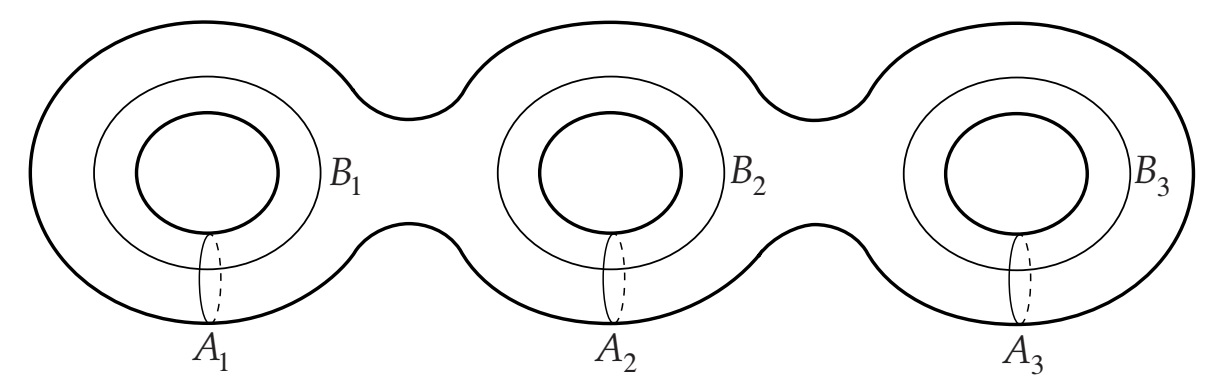
\includegraphics[width=0.8\textwidth,natwidth=852.6,natheight=271.6]{Fig9.1.jpg}\\
		\caption{Fig. 9.1. Genus-three surface with $A$ - and $B$ -cycles marked.}\label{Fig9.1}
	\end{center}
\end{figure}

它们是非平庸曲线,即无法收缩到一点. 如果我们横穿其中一条曲线,在覆盖空间上我们不回到原点而是等价于它的曲线,因此对于每个闭链,我们赋予 $P S L(2, \mathbf{R})$的一个元素,也记为 $A_{i}$或 $B_{i}$.\\
$A$ 闭链和$B$ 闭链是完备的,在每个闭合路径都同伦 (homotopic)等价于一连串的 $A$ 闭链或 $B$闭链. 事实上,它们是过完备的:路径
\begin{equation}
	\left(A_{1} B_{1}^{-1} A_{1}^{-1} B_{1}\right)\left(A_{2} B_{2}^{-1} A_{2}^{-1} B_{2}\right) \ldots\left(A_{g} B_{g}^{-1} A_{g}^{-1} B_{g}\right)
\end{equation}
可收缩到一点,并且相应乘积必须是单位元. 对模计数,在每个 $P S L(2, \mathbf{R})$ 元素中有6个实参量,给出$6 g$, 从约束 $(9.2 .4)$中减去3个. 由于总的$P S L(2, \mathbf{R})$ 给出等价曲面,再减去3个,总共$6 g-6$ .\\
尽管Schottky参量化与Fuchsian参量化类似,但它们有相当不同的性质. 特别地,后者的复结构不那么显然,相应地,到超弦的扩张也就不那么简单.

\subsection*{\centerline{The period matrix(周期矩阵)}}
环面的模参量 $\tau$ 在亏格为$g$时可以自然地推广至 $g \times g$ 矩阵. 为看到这一点,我们首先需要 Abelian微分或全纯1-形式. 它们是世界面场 $\omega_{a}$,在复坐标中拥有如下性质
\begin{equation}
	\partial_{\bar{z}} \omega_{z}=0, \quad \omega_{\bar{z}}=0
\end{equation}
精确有 $g$个这样的场,并且 $g$ 进一步满足共轭关系. 这源于Riemann-Roch 定理 (5.3.22).  Abelian 微分 (9.2.5) 及其共轭正是算符 $P_{0}^{T}$的核. 对此,Riemann-Roch定理是
\begin{equation}
	\operatorname{dim} \operatorname{ker} P_{0}^{T}-\operatorname{dim} \operatorname{ker} P_{0}=-\chi=2 g-2
\end{equation}
算符 $P_{0}$ 作用在 $h=0$的标量场 $c$和$\tilde{c}$上,因而退化至普通的梯度. 这总有2个零模 (c= constant or $\tilde{c}=constant$  ), 因而 dim ker $P_{0}^{T}=2 g$.\\
1-形式的线积分是坐标不变量. 那么Abelian微分的自然基就是 $\omega_{z i}, i=1, \ldots, g$, 定义成
\begin{equation}
	\oint_{A_{i}} d z \omega_{z j}=\delta_{i j}
\end{equation}
那么周期矩阵
\begin{equation}
	\tau_{i j}=\oint_{B_{i}} d z \omega_{z j}
\end{equation}
表征了曲面的复结构. 当亏格为1时, $\omega_{z}$ 是常数,这是通常的$\tau$.\\
可以证明 $\tau_{i j}$是对称的,所以它有 $\frac{1}{2} g(g+1)$ 个复参量. 当 $g=1,2,3$ 它等于复模的个数. 当 $g \geq 4$ 时,它会大一些,所以不是所有周期矩阵都对应Riemann面. theta函数 (7.2.36) 有一个自然的亏格-g推广. 那时 $\tau$ 变成周期矩阵, $v, n, a, b$ 变成 $g$分量矢量.\\

\subsection*{\centerline{Hyperelliptic surfaces(超椭圆曲面)}}
还有一种描述,有时是非常有用的. 考察空间 $S_{2} \times S_{2}$, 坐标分别为 $z$ , $y$. 考察如下方程给定的子流形
\begin{equation}
	y^{2}=\prod_{i=1}^{2 k}\left(z-Z_{i}\right)
\end{equation}
$Z_{i} $是复参量. 投射到 $z$坐标上,存在$k$ 个割线相连的两个曲面. 这给出有 $g=k-1$ 个柄的曲面. 当投射到 $z$时,支点是奇异的,但整个曲面 (9.2.9)不奇异: $y$是定域好坐标.\\
这个曲面依赖$2 k$ 个复$Z_{i}$, 但其中一些在 Möbius变换下冗余,留下 $2 k-3=2 g-1$个复参量. 当 $g=1,2$,这与模的个数相同;但 $g \geq 3$ 时,模的个数更多一些,只有特殊的曲面有 (9.2.9)的形式,它们被称为超椭圆曲面.

\section{世界面的缝合与切割}%{9.3 Sewing and cutting world-sheets}
在分析弦振幅时,一个有用的概念是高亏格振幅与低亏格振幅之间的关系. 其中的关键要素是排水管(plumbing
fixture). 这用来用低亏格曲面构建高亏格曲面. 考察两个世界面 $M_{1}$ , $M_{2}$,坐标分别为 $z_{1}$ , $z_{2}$. 我们可以连接它们构成新的世界面 $M$ . 方法如下:令 $q$是复参量. 从 $M_{1}$ 上减掉圆盘 $\left|z_{1}\right|<(1-\epsilon)|q|^{1 / 2}$ ,从 $M_{2}$ 减掉 $\left|z_{2}\right|<(1-\epsilon)|q|^{1 / 2}$,$\epsilon$为一小量. 为了构成一个面,等同点,使得
\begin{equation}
	z_{1} z_{2}=q
\end{equation}
如图\ref{Fig9.2}所示. 

\begin{figure}
	\begin{center}
		%width=0.8\textwidth,bb=0 0 877 729
		%1px=0.75pt
		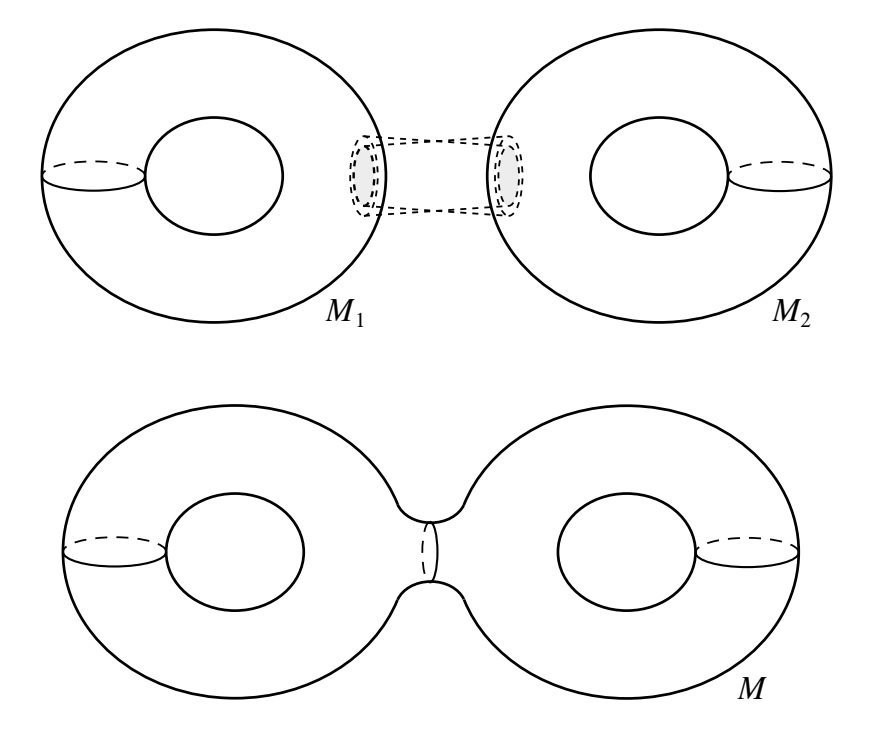
\includegraphics[width=0.8\textwidth,natwidth=613.9,natheight=530]{Fig9.2.jpg}\\
		\caption{Fig. 9.2. Joining two world-sheets by removing a disk (shaded) from each and gluing the edges as indicated by the dashed lines.}\label{Fig9.2}
	\end{center}
\end{figure}

圆盘区域
\begin{equation}
	(1-\epsilon)^{-1}|q|^{1 / 2}>\left|z_{1}\right|>(1-\epsilon)|q|^{1 / 2}
\end{equation}
像图中所示的那样缝合在一起. 这一构造的一个表示是
\begin{equation}
	M=M_{1} \infty M_{2}\left(z_{1}, z_{2}, q\right)
\end{equation}
 这个符号强调了相应表面依赖于定域坐标的选择. 若选择相同的定域坐标$z_{1}^{\prime}$ 和 $z_{2}^{\prime}$,将会剪掉不同的圆,并且连接曲面一般不同. 这两个坐标卡也可能处在单个曲面$M_{0}$的不同部分. 那么排水管构造给曲面加了一个柄. 这记为
\begin{equation}
	M=M_{0} 8\left(z_{1}, z_{2}, q\right)
\end{equation}
符号' $\infty$ ' 和 ' 8 ' 用来区分两种缝合过程. 参量$q$实际上是不需要的————取$z_{1}^{\prime}=z_{1} q^{-1 / 2}, z_{2}^{\prime}=$ $z_{2} q^{-1 / 2}$, 和 $q^{\prime}=1$ 给出等价曲面. 引入$q$ 是为了方便讨论坐标卡固定时,随着$q$ 变化的行为.\\
我们也可以逆转这一构造. 给定任意的Riemann面 $M$, 以及上面的不相交曲线 $C$ ,总可以在$C$的邻域内找到全纯坐标得$z_{1}=z_{2}^{-1}$,使得 $C$由 $\left|z_{1}\right|=\left|z_{2}\right|=|q|^{1 / 2}$给出. 剪切 $C$ (撤销等价关系 $\left.z_{1} z_{2}=q\right)$ 并粘回圆盘$\left|z_{1}\right|<|q|^{1 / 2}$ 和 $\left|z_{2}\right|<|q|^{1 / 2}$ ,这产生了 $M_{1}$和 $M_{2}$ (或 $M_{0}$ ),使得 $M$ 可以通过缝合操作重新产生. 取决于剪切$C$是否使得曲面非连通,我们分别使用缝合 (9.3.3) 或 (9.3.4) .\\
对于图\ref{Fig9.2}中亏格为2的例子,考察$q \ll 1$的情况. 图\ref{Fig9.3}a给出了这一情况下的 $M$. 

\begin{figure}
	\begin{center}
		%width=0.8\textwidth,bb=0 0 994 578
		%1px=0.75pt
		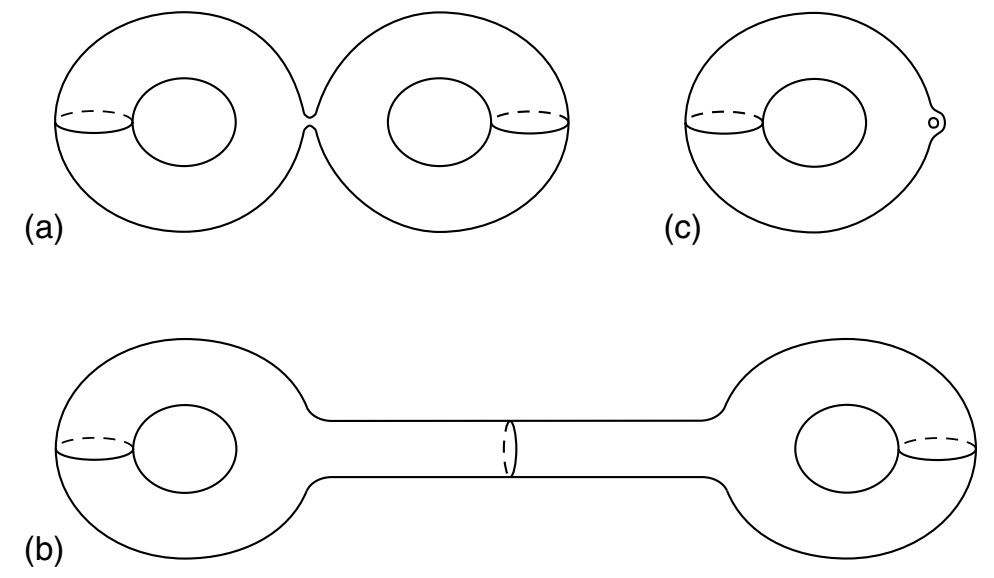
\includegraphics[width=0.8\textwidth,natwidth=695.8,natheight=420]{Fig9.3.jpg}\\
		\caption{Fig. 9.3. Three representations of the genus two surface with degenerating cycle.}\label{Fig9.3}
	\end{center}
\end{figure}

在重叠区域,w偶们已经在$d z_{1} d \bar{z}_{1}$ 和 $d z_{2} d \bar{z}_{2}$之间光滑地插入了度规,曲面被捏成了半径量级为 $|q|^{1 / 2} $ 的圆. 通过一个Weyl变换,总可以找到一个度规,使得半径保持量级为1,如图\ref{Fig9.3}b所示. 既然 Weyl 变换的作用是等距的,其效应是柄的长度变得很大,量级欸$-\ln |q| $. 柄区域$\left|z_{1}\right|<1,\left|z_{2}\right|<1$ 等效于圆柱
\begin{equation}
	\ln |q|<\operatorname{Im} w<0, \quad w \cong w+2 \pi
\end{equation}
其中 $z_{1}=\exp (-i w)$ and $z_{2}=q \exp (i w) $. 图\ref{Fig9.3}c给出了同一曲面的另一表示. 围绕小柄周围的圆盘区域 $O(|q|)<|z|<O(1)$共形等价于图\ref{Fig9.3}b的长圆柱. 以图\ref{Fig9.3}a的形式,可以认为这一图景是所有 $M_{2}$ 都已约化的Weyl变换.\\
在所有这些图景中,显然曲面在 $q \rightarrow 0$的极限下变得特殊. 这个柄称为尖点(pinch)或退化(degenerate). 这是模空间边界的一个例子. 模空间边界非常重要,因为每个发散必须来源于此. 事实上,我们将看到每个边界都是这样的形式,一个或多个柄箍缩了(pinches).  对于亏格-2的曲面,有另外一种单个柄退化的方式. $A$ 闭链或 $B$ 闭链箍缩. 这分别对应于从单个环面出发经由 ' 8 '操作(而非从两个环面出发经由' $\infty$ ' 操作) 构建亏格-2的环面并取 $q \rightarrow 0$.\\
通过重复使用剪切操作,我们会发现一个有趣的事实,每个Riemann面会退化成有3个小孔的球面. 一个小孔是一个标记点,在这个点附近有一个特定的复坐标;这是在排水管缝合时所需的数据. 换句话说,每个Riemann面可以从有3个小孔的球面出发经由缝合构造. 例如,图\ref{Fig9.4}给出了3种构造有4个顶点算符的亏格2曲面的方法. 对于每个缝合操作有一个复模 $q$. 对于图\ref{Fig9.4}中的每个构造,这给出了7个单复模. 这些对应于亏格为2的曲面的 $3 g-3=3$个复模加上4个顶点算符的位置.

\begin{figure}
	\begin{center}
		%width=0.8\textwidth,bb=0 0 954 553
		%1px=0.75pt
		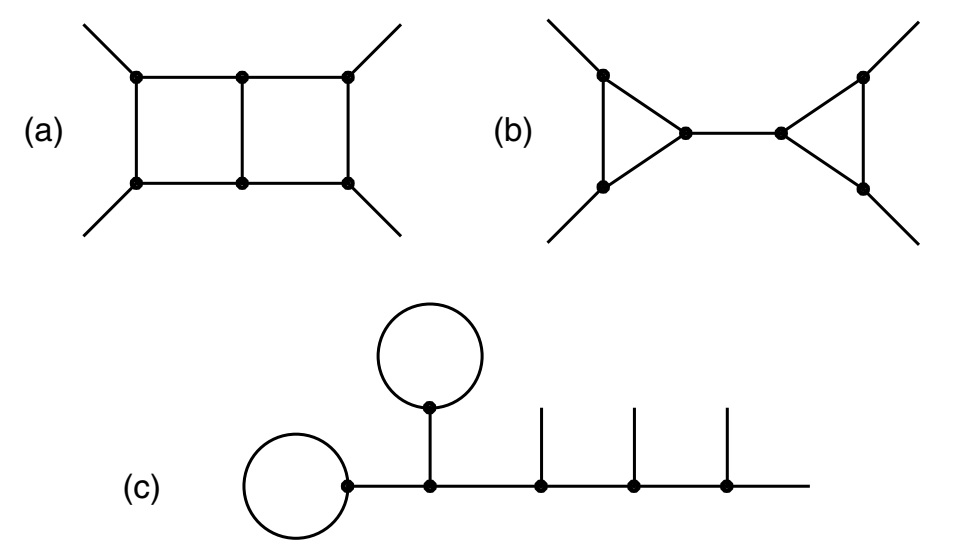
\includegraphics[width=0.8\textwidth,natwidth=667.8,natheight=414.75]{Fig9.4.jpg}\\
		\caption{Fig. 9.4. Some sewing constructions of the genus-two surface with four operators. Each vertex is a sphere with three punctures, each internal line represents the plumbing fixture construction, and each external line represents a vertex operator.}\label{Fig9.4}
	\end{center}
\end{figure}

\subsection*{\centerline{A graphical decomposition(图论分解)}}
图\ref{Fig9.4}让人联想到Feynman图. 我们现在来描述模空间的Feynman-diagram-like 分解. 顶点要比\ref{Fig9.4}复杂得多,可以有任意多外线以及弦圈中的内部修正. 这一构造的关键在于让模空间边界的性质变得显然.\\
陈述如下:对模空间的积分由Feynman图的和给出. 图中的内线传播子代表缝合操作,要积掉的缝合参量 $q$ 处在某些标准区域中,例如$|q|<1 $ .  $n$ 点顶角代表有 $n$个小孔的Riemann面. 我们将会看到顶点中的曲面要对模空间的某个内部积分,并对亏格求和. 缝合操作是指对要缝合的每个点指定复坐标,所以顶角的定义必须包含在每个点的选择. 在$n$点顶角出现的亏格g的曲面集合记为 $\mathscr{V}_{g, n} $ . 外线代表顶点算符.\\
我们举例说明这一构造. 从三点顶角 $\mathscr{V}_{0,3}$出发,如图\ref{Fig9.5}所示. 它是有3个标记点和3个缝合圆的球面. 

\begin{figure}
	\begin{center}
		%width=0.8\textwidth,bb=0 0 343 313
		%1px=0.75pt
		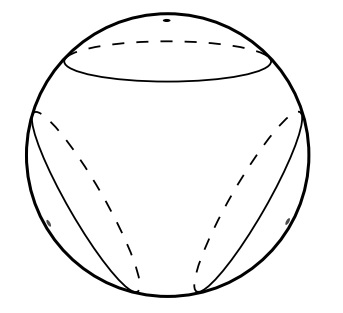
\includegraphics[width=0.4\textwidth,natwidth=257.25,natheight=234.75]{Fig9.5.jpg}\\
		\caption{Fig. 9.5. Trilinear string vertex, with three marked points and three sewing circles on the sphere.}\label{Fig9.5}
	\end{center}
\end{figure}

在相应点附近的复坐标中,缝合圆是单位圆. 建立有4个点的球面的步骤:取两个这样的顶角,各移掉一个缝合圆的内部,然后将它们粘在一个圆柱两端;这等价于排水管构造. 这对应于图\ref{Fig9.6}a的
Feynman图;圆柱的长度为$-\ln |q| $(周长调整为 $2 \pi$ ). 对 $|q|<1$ 积分,并对其他两个道求和仅给出有四个点的球面的一部分积分区域,如图\ref{Fig9.6}b所示. 阴影区域被囊括在内,非阴影区域却消失了.

\begin{figure}
	\begin{center}
		%width=0.8\textwidth,bb=0 0 987 482
		%1px=0.75pt
		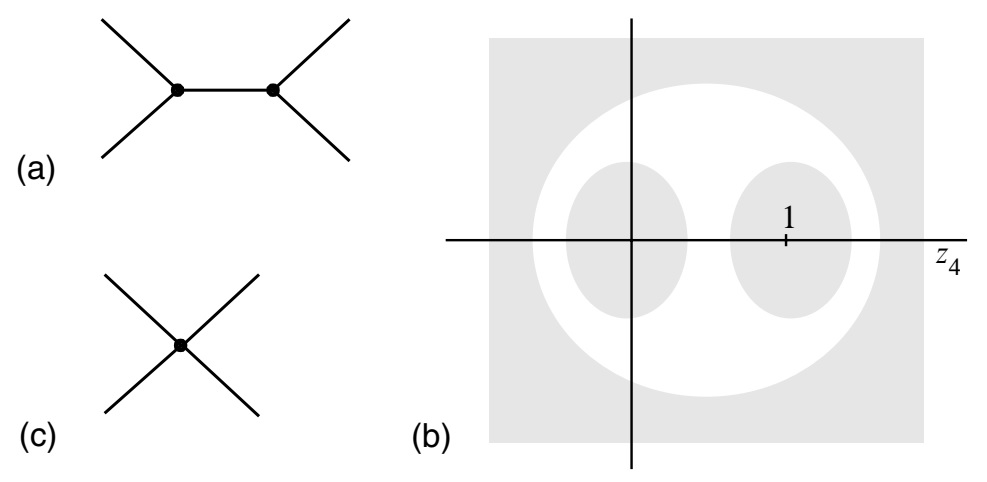
\includegraphics[width=0.8\textwidth,natwidth=740.25,natheight=361.5]{Fig9.6.jpg}\\
		\caption{Fig. 9.6. (a) Constructing the sphere with four vertex operators. (b) The region of the $z$ -plane covered by this graph. (c) The additional vertex needed to give the correct amplitude. The four-punctured sphere is integrated over the unshaded region.}\label{Fig9.6}
	\end{center}
\end{figure}

我们来做进一步的解释. 对于三线性顶角,将点放在球面的 $0,1, \infty$ 处,并选择坐标系 $z^{(0)}, z^{(1)}$, $z^{(\infty)}$ ,所以三个缝合圆是 $\left|z^{(0,1, \infty)}\right|=1$. 选择应该在置换顶角的6个Möbius 变换下不变. 这使得顶角是对称的. 存在多个可能的选择,例如
\begin{equation}
	z^{(0)}=\frac{a z}{z-2}, \quad z^{(1)}=\frac{a(z-1)}{z+1}, \quad z^{(\infty)}=\frac{a}{2 z-1}
\end{equation}
其中$a$为任意常数. 当$a \geq 3$时,缝合圆不会重合,保证了对于所有 $q \leq 1$排水管构造都给出好曲面. 读者可以证明,从两个球面,在参量 $q$ 下缝合$z^{(\infty)}$与 $z^{(0)}$ 坐标卡给出顶点算符在 $0,1, \frac{1}{2}\left(1+a^{2} / q\right)$和 $\frac{1}{2}\left(1-a^{2} / q\right) $ 的球面. 在Möbius变换下,这等价于顶点算符在$0,1, \infty$, 以及
\begin{equation}
	z_{4}=\left(q-a^{2}\right)^{2} / 4 a^{2} q
\end{equation}
随着 $q$跑遍单位圆盘, $z_{4}$ 覆盖了图\ref{Fig9.6}b的外部阴影区域. 置换顶点给出其他两个区域. 我们可以尝试取更小的$a$,这样阴影区域会增长,但它们最终会重合,并对某些曲面二次计数. 而另一些曲面仍然不会产生. 它们永远不会精确覆盖整个平面. 所以我们还要添加一个显式的四点顶角 $\mathscr{V}_{0,4}$ ,它由有4个标记点的球面给出,并对 $z$ 平面的非阴影区域积分. 由于对于$z_{4} $的每个值,对每个孔的坐标还有一个选择,这无法完全定义 $\mathscr{V}_{0,4}$,以光滑的方式连接阴影区域的边界和非阴影区域的边界. 注意到图\ref{Fig9.6}a的 Feynman图包含所有渐近区域 $z_{4} \rightarrow 0,1, \infty$, 而四点顶角只包含非退化曲面,那么这一极限下的行为显然由$q \rightarrow 0$ 的极限给出. 这是为什么排水管构造有用的原因.\\
作为一个例子,将单个顶角的两个圆缝合在一个圆柱的两端,这给出有一个顶角算符的环面. 这覆盖了环面模空间的$\operatorname{Im} \tau \rightarrow \infty$ 极限,但内部区域丢失了,必须通过手加顶角区域 $\mathscr{V}_{1,1}$补回来.\\
这个构造可以诱导地扩张. 缝合操作总会增加参量
\begin{equation}
	r=3 g+n-2
\end{equation}
有三个小孔的原始球面,顶角$\mathscr{V}_{0,3}$, 有 $r=1$. “8”操作给出 $r=r_{0}+1$, 而 $\infty$ 操作给出$r=r_{1}+r_{2}$. 因此, $\mathscr{V}_{0,4}$ 和 $\mathscr{V}_{1,1}$ 均有$r=2$. 已经证明通过 $r$的诱导可以构造出 $\mathscr{V}_{g, n}$ ,因此如同之前宣称的,覆盖了整个模空间.\\
下面给出一个更加清晰的构造. 在任意Riemann面上,存在唯一的最小面积度规,它的定义是,最小面积的度规服从约束使得每个不平庸的闭合曲线的长度至少为 $2 \pi$. 这个曲面上的每个点至少处在一条饱和测地线上(saturating geodesic),一条长度精确为$2 \pi$非平庸闭合曲线. 可以连续变换到其他饱和测地线的饱和测地线不会自相交,每组同伦等价的饱和测地线构成曲面上的一个环 (拓扑上是圆环) . 不同的环会覆盖整个曲面,但可能会有重叠. 这种环的高$h$定义为它的两个边界测地线之间的最短距离. 最小面积度规的思想可以扩展至有小孔的曲面. 方法是,围绕小孔的圆不是平庸的. 小孔附近的最小面积度规形式为 $d z d \bar{z} / z \bar{z}$, 一个半径 $2 \pi $ 的半无限长圆柱. 因此存在两类环,一类有限处在曲面内部,另一类非无限长汇集在小孔处,终结于曲面内部.\\
我们现在可以用这种构造描述 $\mathscr{V}_{g, n}$. 取有$n$个小孔的所有Riemann面,赋予约束,任何内部环的高度在最小面积度规下小于 $2 \pi $ . 截断半无限长圆柱,留下长度为$\pi$的存根(stub),并粘入通常的圆盘中,在存根的底部插入顶点算符. 有了这些顶角,Feynman图之和会精确地一次性覆盖模空间. 可以证明,缝合最小面积曲面仍然会产生最小面积曲面. 高度小于$2 \pi$的环显然包含在顶角中,高度大于$2 \pi$ 的环会由存根上的缝合算符产生,相应高度是存根的$2 \pi$ 加上排水管的$-\ln |q|$ ; 当对$q$ 积分时,这从$2 \pi$跑到 $\infty$. 最小长度约束与最大高度保证了生成的曲面会出现在顶角中,所以仅当一个或多个$q$趋于零时才会产生,这正是所要证明的.

\section{共形场论中的缝合与切割}%{9.4 Sewing and cutting CFTs}
通过将低亏格Riemann面缝合在一起,我们描述了高亏格Riemann面. 利用路径积分的缝合性质,类似地,高亏格曲面上的CFT可以与低阶振幅相关联. 这个关系如图\ref{Fig9.7}所示.

\begin{figure}
	\begin{center}
		%width=0.8\textwidth,bb=0 0 957 668
		%1px=0.75pt
		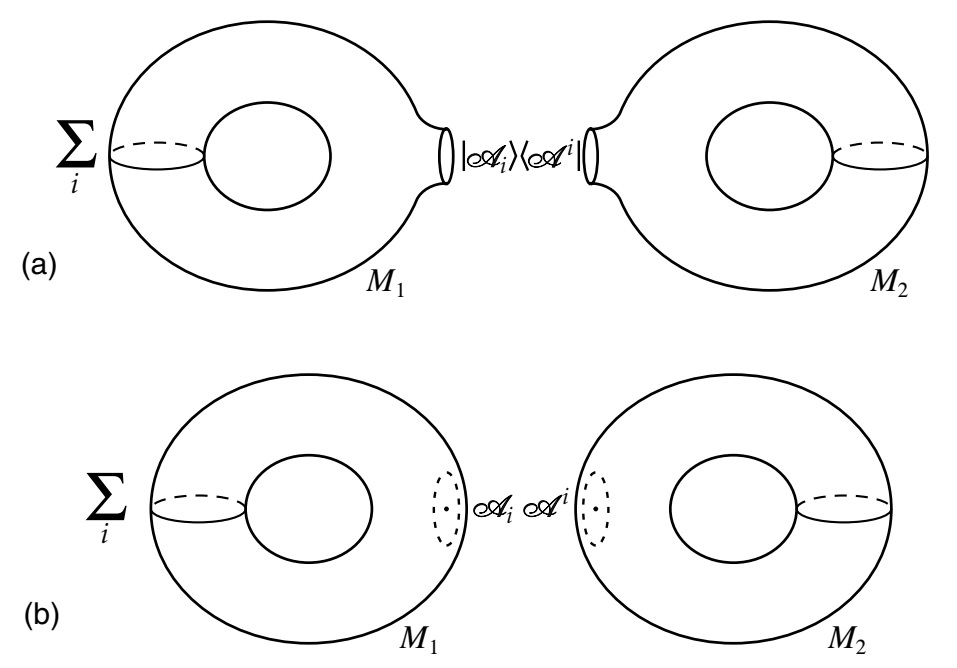
\includegraphics[width=0.8\textwidth,natwidth=717.75,natheight=501]{Fig9.7.jpg}\\
		\caption{Fig. 9.7. (a) The path integral on $M$ is cut open by inserting a complete set of boundary states. (b) Each state is replaced by a disk with local operator.}\label{Fig9.7}
	\end{center}
\end{figure}

为明晰起见,我们首先讨论 $q=1 $的情况.  $M$上的路径积分沿着圆 $\left|z_{1}\right|=\left|z_{2}\right|=1$剪开,插入边界态的完备集. 那么每个边界态就被替换成有相应定域算符的圆盘,留下未裁剪的世界面 $M_{1}$ 和 $M_{2}$. 这个结果的精确形式是
\begin{equation}
	\left\langle\ldots_{1} \ldots_{2}\right\rangle_{M}=\sum_{i j}\left\langle\ldots \mathscr{A}_{i}^{\left(z_{1}\right)}\right\rangle_{M_{1}} \mathrm{G}^{i j}\left\langle\mathscr{A}_{j}^{\left(z_{2}\right)} \ldots 2\right\rangle_{M_{2}}
\end{equation}
我们允许在$M_{1}$和$M_{2}$上有任意额外的插入 $\ldots 1$ 和 $\ldots 2$ ; 它们必须处在圆 $\left|z_{1}\right|=1$ 和$\left|z_{2}\right|=1$ 外面. 我们还没有为这组基指定任何特定的正交性;仍需决定合适的可逆矩阵 $\mathrm{G}^{i j}$ . 代替柄的插入 $\mathscr{A}_{i}$ 和 $\mathscr{A}_{j}$ 分别隐含在 $z_{1}$ 和 $z_{2}$ 坐标系的原点中.\\
现在,我们来考察 $M_{2}$是球面的情况. 将缝合坐标 $z_{2}$ 记作$u$,$\ldots 2$是$z=0 $处的定域算符 $\mathscr{A}_{k}$. 我们从排水管构造中有 $z_{1} u=1$ ,从球面中有 $z u=1$ ,所以我们可以将 $z_{1}=z$ 扩张至整个缝合区域. 缝合曲面 $M$ 与 $z_{1}=0$处有一额外算符$\mathscr{A}_{k}$ 的 $M_{1}$相同. 那么 (9.4.1) 变成
\begin{equation}
	\left\langle\ldots 1 \mathscr{A}_{k}^{\left(z_{1}\right)}\right\rangle_{M_{1}}=\sum_{i j}\left\langle\ldots 1 \mathscr{A}_{i}^{\left(z_{1}\right)}\right\rangle_{M_{1}} \mathbf{G}^{i j}\left\langle\mathscr{A}_{j}^{(u)} \mathscr{A}_{k}^{(z)}\right\rangle_{S_{2}}
\end{equation}
两点函数 $\left\langle\mathscr{A}_{j}^{(u)} \mathscr{A}_{k}^{(z)}\right\rangle_{S_{2}}$ 正是内积 $\left\langle\langle j \mid k\rangle=\mathscr{G}_{j k}\right.$ . 那么(9.4.2) 暗示了
\begin{equation}
	\mathbf{G}^{i j} \mathscr{G}_{j k}=\delta_{k}^{i}
\end{equation}
或者
\begin{equation}
	\mathrm{G}^{i j}=\mathscr{G}^{i j}
\end{equation}
即,球面上的两点函数定义的内积正是缝合所需要的. 因此,针对$M_{2}$是含有一个任意定域算符的球面,我们导出了 (9.4.1) . 通过态-算符同构,任何边界态可以以这种方式获得. 既然路径积分是平庸的,这个结果只依赖缝合区域,但与曲面的其余区域无关,所以它对于任意的 $M_{2}$ 和$\ldots 2$都成立.\\
用参量 $q$进行缝合与用 $q=1$以及定域坐标 $z_{1}$和 $z_{2}^{\prime}=z_{2} / q $ 进行缝合是等同的. 因此,我们就获得了 $\mathscr{A}_{j}$在带撇坐标系中的(9.4.1). 因而从回到 $z_{2}$的共形变换中获得额外因子,
\begin{equation}
	\mathscr{A}_{j}^{\left(z_{2}^{\prime}\right)}=q^{h_{j}} \bar{q}^{\tilde{h}_{j}} \mathscr{A}_{j}^{\left(z_{2}\right)}
\end{equation}
这个结果是
\begin{equation}
	\langle\ldots 1 \ldots 2\rangle_{M}=\sum_{i j} q^{h_{j}} \tilde{q}^{\tilde{h}_{j}}\left\langle\ldots_{1} \mathscr{A}_{i}^{\left(z_{1}\right)}\right\rangle_{M_{1}} \mathscr{G}^{i j}\left\langle\mathscr{A}_{j}^{\left(z_{2}\right)} \ldots 2\right\rangle_{M_{2}}
\end{equation}
其中我们取了关于权重对角的基. 对于 ' 8 ' 操作, $M$ 和$M_{0}$ 上的路径积分以相同方式关联
\begin{equation}
	\langle\ldots\rangle_{M}=\sum_{i j} q^{h_{j}} \bar{q}^{\tilde{h}_{j} c g^{i j}}\left\langle\ldots \mathscr{A}_{i}^{\left(z_{1}\right)} \mathscr{A}_{j}^{\left(z_{2}\right)}\right\rangle_{M_{0}}
\end{equation}
再次考察模空间的边界,它由一个或多个柄的$q \rightarrow 0$给出. 我们看到低权重算符将会控制这个行为.  (9.4.6) 与 (9.4.7) 类似于OPE,实际上,当$M_{2}$是球面,并且 ${}_{\cdots 2}$是一对顶点算符,  $(9.4 .6)$会退化至OPE. 这个类比从图\ref{Fig9.3}c看是显然的,它将这个极限表示成了插入了小柄. 缝合关系表明不只算符乘积,或者一个小柄,或者我们可以缝合进小圆的任何扰动,均等价于定域算符的和. 
(9.4.6) 是OPE的漂亮推广. 从 $M_{1}$的观点来看,有一份很小的 $M_{2}$ 粘在 $z_{1}=0$附近. 这可以用定域算符 $\mathscr{A}_{i}$展开,系数函数是 $\left\langle\mathscr{A}^{i} \ldots 2\right\rangle_{M_{2}}$ . 以 $M_{2}$的观点看,有一份细小的$M_{1}$ 粘在 $z_{2}=0$附近,它可以用 $\mathscr{A}^{i}$展开,系数函数是 $\left\langle\ldots 1 \mathscr{A}_{i}\right\rangle_{M_{1}}$.\\
我们已经论证了每个Riemann面可以退化至带3个小孔的球面. 因此,缝合构造将所有振幅与球面上的三点振幅关联起来,而它们显然是算符乘积系数:它们是定义CFT的数据. 我们会遇到很多CFT之间的等价性————我们已经看到了T对偶,而玻色化将是另一个值得注意的例子. 缝合构造提供了两个理论是否相等的判据:它们的态和恒等OPE之间的一一映射. 
\footnote{ We should note that when there is more than one $(2,0)$ plus $(0,2)$ field that could play the role of $T_{a b}$, as in the free-field examples of section $2.5$, it is necessary to specify which is the energy-momentum tensor. This choice determines the conformal transformations of operators, which enter implicitly into the sewing relation.}
事实上,我们会在第15章证明,仅初级场的算符乘积就决定了所有其他场的算符乘积. \\
我们来进一步探索这个观点. 我们可以沿着各种不同的曲线剪开一个曲面,所以为了保证缝合关系,对于$M$上的期望值总给出相同的结果. 首先考察剪切曲线 $C$上的无穷小变换. 一般使得$M$不变的无穷小变换可以通过对用于缝合的坐标做无穷小变换获得
\begin{subequations}
\begin{equation}
		z_{1}^{\prime}=z_{1}+\sum_{n=-\infty}^{\infty} \epsilon_{n} z_{1}^{n+1} 
\end{equation}
\begin{equation}		
		z_{2}^{\prime}=z_{2}-\sum_{n=-\infty}^{\infty} \epsilon_{-n} q^{-n} z_{2}^{n+1}
\end{equation}
\end{subequations}
那么缝合表达式的差会正比于
\begin{equation}
	\begin{aligned}
		\mathscr{A}_{i}^{\left(z_{1}^{\prime}\right)} \mathscr{G}^{i j} \mathscr{A}_{j}^{\left(z_{2}^{\prime}\right)}-\mathscr{A}_{i}^{\left(z_{1}\right)} \mathscr{G}^{i j} \mathscr{A}_{j}^{\left(z_{2}\right)}=&-\sum_{n=-\infty}^{\infty} \epsilon_{n}\left[L_{n} \cdot \mathscr{A}_{i}^{\left(z_{1}\right)} \mathscr{G}^{i j} \mathscr{A}_{j}^{\left(z_{2}\right)}\right.\\
		&\left.-\mathscr{A}_{i}^{\left(z_{1}\right)} \mathscr{G}^{i j} L_{-n} \cdot \mathscr{A}_{j}^{\left(z_{2}\right)}\right]+\text { (anti) }
	\end{aligned}
\end{equation}
其中我们使用了共形变换 (2.9.6), 而 'anti'代表将 $\epsilon_{n} \rightarrow \epsilon_{n}^{*}$ ,并将 $L_{n} \rightarrow \tilde{L}_{n} $ . 通过用来推导 (9.4.4)的讨论可以证明大括号中的量. 这相当于说明我们可以将定义生成元的围道积分拉过缝合柄. 从$L_{n}$ 到 $L_{-n}$ 的变化来自于坐标的反转. 所有其他的守恒荷围道积分也可以拉过来.\\
还有一些曲线的集合无法通过连续变换关联起来. 通过剪切围绕不同对算符的圆,球面上的四点振幅可写成三点振幅的形式. 不同缝合之间的等价性是OPE结合律的结果,见图2.8.\\
另一个例子由环面给出:通过沿着$A$ 闭链或 $B$闭链,或者任何其他不自交的闭合曲线剪切,我们可以使环面退化至球面. 以带有等价关系的平面来讲,始于 $\left(\sigma^{1}, \sigma^{2}\right)=(0,0)$的闭合曲线  $C$ 必须结束于等价点
\begin{equation}
	2 \pi(m, n)
\end{equation}
所有 $m$ 和 $n$值相同的曲线可以连续地变换到彼此,所以我们需要考察沿着 $m$和$n $不同的曲线缝合之间有什么关系. 可以证明,对于非平庸的不自交曲线,$m$ 和 $n$ 必须互素,这暗示了存在整数 $p$ 和$q$,使得 $m p-n q=1 $. 那么存在另一个模变换
\begin{equation}
	\left(\sigma^{1}, \sigma^{2}\right)=\left(\sigma^{\prime 1}, \sigma^{\prime 2}\right)\left[\begin{array}{cc}
		m & n \\
		q & p
	\end{array}\right]
\end{equation}
使得曲线 $C$ 回到
\begin{equation}
	\left(\sigma^{\prime 1}, \sigma^{\prime 2}\right)=2 \pi(1,0)
\end{equation}
这是$A$ 闭链. 所以沿着非平庸不自交曲线剪切等同于在 $\tau $的一个模等价值上沿着 $A$ 闭链剪切. 因此,缝合构造的相容性就等价于模不变性.\\
通过连续的两移(two moves),每组缝合曲线可以变换到彼此:球面上的四点组合变换,以及含有一个顶点算符的环面上的模变换. 图\ref{Fig9.4}使其相当可信. 例如,图\ref{Fig9.4}a通过一个结合性条件与图\ref{Fig9.4}b相关. 重复利用结合性可以将缝合带至图\ref{Fig9.4}c的形式,这时所有圈都表示成了单圈单点函数. 所以,它们是定义一个合理的共形场论任意一组算符乘积系数的条件. 这种用来解决对偶约束的程式被称为共形自举(conformal bootstrap). 仅在引入额外约束的情况下,这才得以实现. 我们将在第15章进行讨论.\\
这一节的考察可以扩展至有边界的世界面. 除了退化柄以外,那里还会有退化带. 相容性条件已经推广至这一情况.

\section{一般的振幅}%{9.5 General amplitudes}
我们现在已经集齐了理解一般弦振幅的相容性所需要的所有元素. 在给定模空间的图形分解后,缝合理论使得我们可以给出一般弦振幅的图形表示. 首先考察来自排水管构造的传播,模 $q$ 的鬼插入是
\begin{equation}
	\left.\oint \frac{d z}{2 \pi i} b_{z_{1} z_{1}} \frac{\partial z_{1}}{\partial q}\right|_{z_{2}}=\frac{b_{0}}{q}
\end{equation}
类似地,对于 $\bar{q}$ 则是 $\tilde{b}_{0} / \bar{q}$. 引入这些插入,并使用缝合表达式(9.4.6), 传播子附带的因子是
\begin{equation}
	\int_{|q|<1} \frac{d^{2} q}{q \bar{q}} q^{\alpha^{\prime}\left(k_{i}^{2}+m_{i}^{2}\right) / 4} \bar{q}^{\alpha^{\prime}\left(k_{i}^{2}+\tilde{m}_{i}^{2}\right) / 4} \mathscr{G}^{i j} b_{0} \tilde{b}_{0}=\frac{8 \pi \delta_{m_{i}^{2}, \tilde{m}_{i}^{2}} \mathscr{G}^{i j} b_{0} \tilde{b}_{0}}{\alpha^{\prime}\left(k_{i}^{2}+m_{i}^{2}-i \epsilon\right)}
\end{equation}
通过在缝合构造的顶点中出现的曲面上插入顶点算符,就给出了$n$ 弦耦合
\begin{equation}
	g\left(i_{1}, \ldots, i_{n}\right)=\sum_{g} \int_{\mathscr{V}_{g, n}} d^{m} t\left\langle\prod_{k=1}^{m} B_{k} \prod_{l=1}^{n} \hat{\nu}_{i_{l}}\right\rangle_{g}
\end{equation}
其中$m=6 g+2 n-6$ 是模的数目. 那么从耦合 (9.5.3) 和传播子 (9.5.2) 构造出的 Feynman 图重新产生了整个弦振幅. 指标$i$ 依旧代表每个弦的态和动量. 9.1节中的树图振幅例证了这一结果.\\
第一个议题是振幅的有限性. 我们断言,发散只能来自于空间的边界. 就像各种低阶振幅中发生的那样. 在模的有限值处,缝合公式给出的是对无限个弦态求和,但由于这个求和根本上是一个量子态在一个完备基中的展开,所以这个求和是收敛的. 实际上,收敛性仅在幺正CFT中才能得以保证,但是,弦CFT的非幺正部分是相当驯服的. $X^{0}$ CFT 是通过从幺正CFT解析延拓定义的  ,而鬼CFT仅仅生成了Faddeev-Popov行列式,所以是有限的. 现在边界作为各种传播子的  $q \rightarrow 0$极限变得显然. 而积分 $(9.5 .2)$在前面遇到过数次. 它是经由解析延拓定义的,给出了普通场论传播子. 那么唯一的奇异性就是传播子中的极点,它表示了中间态中在壳粒子的产生. 特别地,它们是长程而非短程发散. \\
另一个议题是幺正性,对于四点树图振幅,我们稍详细地探讨了幺正性. 将一般振幅带到Feynman图形式,而不是细致地解出组合性,我们就可以引用标准场论中关于图形表示幺正性的结果. 另外,在9.1节末尾例证了对中间态的求和会退化至对物理态的求和,这一结果会像场论中那样得以推广. \\
作为总结,弦论中的微扰有限性与幺正性所包含议题表现得容易理解. 再次注意到,我们没有假定26个平坦维,而仅是$d$个平坦维加上中心荷为 $26-d$的紧致正范的CFT. 当然,对于玻色弦而言,既然平坦时空不是它的解,任何对于平坦时空S矩阵幺正性的讨论多少有些形式主义————首先存在快子稳定性问题. 其次还有由圈引入的宇宙学常数问题.\\
证明弦论的有限性和幺正性的另一方法基于光锥规范. 这一方法也被极大地发展了. 这个规范放弃了协变性,但它有相当的优势————它使得给出模空间的显式描述变得可能,并且振幅可以表示成场论形式,且Hamiltonian关于光锥时间 $x^{+}$是定域的. 通过证明微扰论等价于协变微扰论,协变性随之建立了 .

\subsection*{\centerline{String divergences(弦发散)}}
在继续前进之前,我们对弦发散是长程发散做进一步解释. 考察带有 $n$个顶点算符的一圈振幅,保持$\tau$不动,取 $m$ 个算符聚在一起的极限,如图\ref{Fig9.8}所示. 

\begin{figure}
	\begin{center}
		%width=0.8\textwidth,bb=0 0 937 514
		%1px=0.75pt
		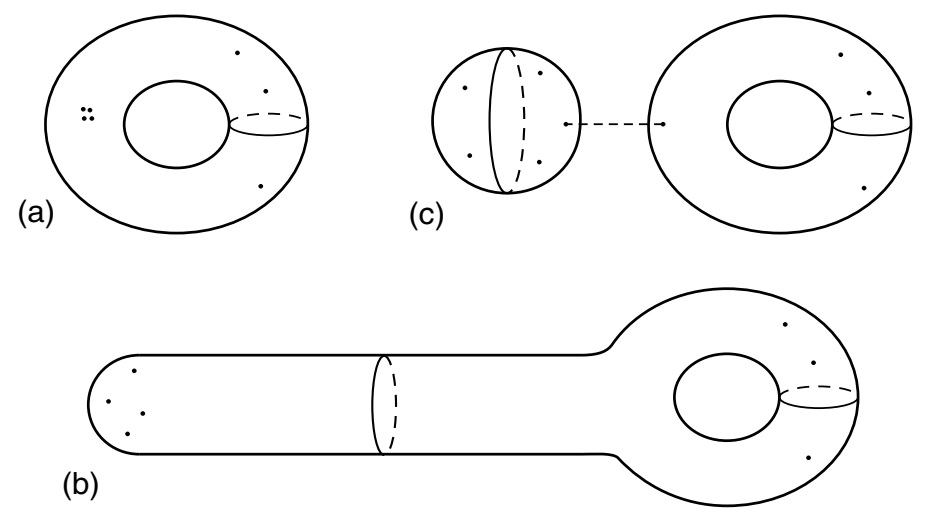
\includegraphics[width=0.8\textwidth,natwidth=702.75,natheight=385.5]{Fig9.8.jpg}\\
		\caption{Fig. 9.8. (a) Torus with $n$ vertex operators, in the limit that $m$ of the operators come together. (b) Conformally equivalent picture: the $m$ vertex operators at the end of a long cylinder. (c) Sewing construction, in terms of the product of a sphere with $m+1$ vertex operators and a torus with $n-m+1$.}\label{Fig9.8}
	\end{center}
\end{figure}

弦圈当然包含引力,当相互作用在时空中聚集时,这有UV发散. 这个弦振幅中确实有发散,但它来自于长程时空距离,而不是短程. 图\ref{Fig9.8}b给出了一个共形等价描述,在那里,$m$ 个顶点算符通过一个长圆柱与剩余的环面相连. 剪开圆柱,并插入态的完备集,我们获得通常的表示 (9.5.2), 而 $q \rightarrow 0$ 变成顶点算符重合的极限. 所以唯一的奇点是传播子在长程时空的极点. 共形不变性再次将世界面上的短程变成时空中的长程.\\
$m=n$和$m=n-1$ 的情况会呈现出特殊问题. 当 $m=n$时,这意味着所有顶点算符都聚集在一起,动量守恒令 $k^{\mu}$为零. 对于无质量态,极点就是 $1 / 0$,由于动量守恒会迫使振幅停留在极点上,所以解析延拓并没有帮助. 这是一个蝌蚪图,就像7.4节中那样,解决方案是相同的. 对背景场的修正,这里的发散正比于带有一个顶点算符的环面振幅.\\
另外一个有问题的情况是 $m=n-1$, 这时除了一个顶点算符 $\mathscr{V}_{n}$外,所有顶点算符都聚集在一起. 动量守恒要求流经圆柱的动量是 $k^{\mu}=-k_{n}^{\mu} $ . 然而,共形不变性要求 $k_{n}^{2}=-m_{n}^{2}$, 所以对于那些$m_{j}^{2}=m_{n}^{2} $ 的中间态,中间态动量被固定在一个极点的顶部,如图\ref{Fig9.9}所示. 

\begin{figure}
	\begin{center}
		%width=0.8\textwidth,bb=0 0 435 233
		%1px=0.75pt
		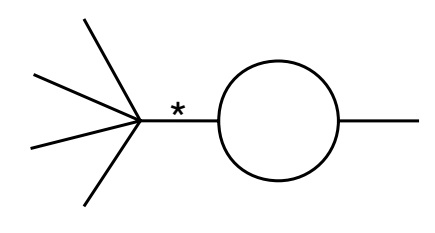
\includegraphics[width=0.8\textwidth,natwidth=326.25,natheight=174.75]{Fig9.9.jpg}\\
		\caption{Fig. 9.9. Field-theory graph analogous to the case $m=n-1$. The kinematics force the starred propagator to diverge. The interpretation is a (finite) mass shift due to the loop.}\label{Fig9.9}
	\end{center}
\end{figure}

中间传播子是 $1 / 0 $ ,只要内线 $j$与外线$n$相同,发散就会发生. 解释是相当简单的,这个圈代表的是对粒子 $n $质量的辐射修正. 定义S矩阵的外动量处在真正的质壳上,其中包括了辐射修正. 并且这依旧没有这个IR发散. 注意到,这里的问题不是圈内的UV发散,而是带星传播子的IR发散. 并且,即使质量修正是有限的,这也会发生. 解决方案在弦情况是相同的. 出现在顶点算符中的动量必须处在真正的物理质量上;一般而言,它们与树图质量并不相同,那些质量的平方是 $1 / \alpha^{\prime}$的整数倍. 注意到,对于特定的无质量场————特别是规范玻色子————规范不变性要求它们在所有阶都是无质量的. 附带地,对于有质量态,质量偏移通常是复的,这些态是不稳定的, 会衰变到轻弦态.\\
这里有一个问题. 早先我们研究弦理论的相容性时,世界面共形不变性要求beta函数 (3.7.14) 为零. 这些beta函数不包括高亏格曲面的信息————它们对应的是树图弦场方程. 当我们试图围绕圈修正背景展开时,会发生什么?事实上,所有问题都迎刃而解了. 图\ref{Fig9.8}中的危险极限不仅给出了发散,也给出了共形反常. 为了看到这点,将这一极限画成\ref{Fig9.3}c中那样,将一个小柄粘在球上. 这个小柄可以用一系列的定域算符表示. 特别地,从无质量能级中有
\begin{equation}
	\partial X^{\mu} \bar{\partial} X_{\mu} \frac{d q d \bar{q}}{q \bar{q}}
\end{equation}
现在通过要求柄的大小大于$a$,即$|q| e^{\omega}>a$, 其中球面上的度规是 $d z d \bar{z} e^{2 \omega} $ ,以坐标不变的方式剪掉发散. 积分$(9.5 .4)$ 的下限给出
\begin{equation}
	-4 \pi \partial X^{\mu} \bar{\partial} X_{\mu} \ln \left(a e^{-\omega}\right)
\end{equation}
因此,我们度规的Weyl因子有了新的依赖:这修正了sigma模型Weyl反常 $\beta_{\mu v}^{G}$ (3.7.14). 为了获得Weyl不变的理论,背景必须满足完整的弦圈修正Weyl不变条件 (或等价的, BRST不变). 来自偏移背景的Weyl反常抵消了来自小柄的反常,这是Fischler-Susskind 机制. 从图\ref{Fig9.3}c,我们可以认为发散和Weyl反常是世界面UV效应,它们并非来自于通常的场的短波涨落,而是来自于非常小的拓扑涨落. 我们应该强调的是,对于亏格任意的固定Riemann面,定域结构是不受拓扑影响的;产生发散和Weyl反常的是对Riemann面的积分. \\
这也可以认为是抵消传播子讨论失效了. 运动学迫使振幅处在极点上,我们无法用解析延拓去消除BRST变分下可能的表面项. 事实上,它们的出现对应于Weyl反常(9.5.5). 在圈修正背景下,来自背景偏移的BRST反常抵消了模空间边界产生的BRST反常,将弦的特性组装在一起给出了相容的时空图景.\\
在弦微扰论中实施这点是相当麻烦的. 但幸运的是,这很少是必要的. 首先,在大多数超对称理论中,背景是不修正的. 其次,在弦论中,对长程物理的分析分成两步是最有效的. 首先用弦论推导出低能有效作用量的形式,然后再长程时使用这个理论. 那么,我们无需处理弦等级的IR发散. 在目前的情况下,蝌蚪图给出了如下的势能项
\begin{equation}
	\delta \boldsymbol{S}=-\sum_{\chi} \Lambda_{\chi} \int d^{d} x(-G)^{1 / 2} e^{-\chi \Phi}
\end{equation}
这里 $\Lambda_{\gamma}$ 是来自Euler数 $\chi$的蝌蚪,而作用量对$\Phi$ 的依赖关系来自于 $e^{\Phi}$是弦耦合. 在经过一番努力后,我们可以从弦振幅中抽取出引力子和伸缩子的各个蝌蚪图.\\
同样的概念扩展至来自质量偏移的顶点算符修正,以及其他的IR发散. 例如,含有无质量粒子理论中的遍举振幅,由于弦论在长程时会退化到场论,这些场论发散也必须出现在相应的弦振幅中. 我们再强调一次,场论中的UV发散一般指出了理论适用范围的基本限制,IR发散通常意味着提出了错误的问题. 任何这样的发散,弦论中的处理方式与场论相同.\\
我们来回顾一下我们学到了什么. 玻色弦特有的模问题,S矩阵有限且幺正,基本机制是模不变性,它截掉了UV发散但没有破坏时空规范不变性. 当然,知道弦理论在围绕平坦时空的弱耦合微扰论中是合理的,这远远不够,我们希望知道超出微扰论,这个理论还是否合理,并有一些计算非微扰修正的手段. 另外,我们希望知道对于时空的短程性质,弦论意味着什么. 在本章的其余部分,我们将简要描述在这些方向上的尝试.

\section{弦场论}%{9.6 String field theory}
比较我们在弦论中使用的方法与构建量子场论的方法是很有趣的. 世界面路径积分类似于对粒子路径求和,这通常称作一次量子化方案. 另一方面,在量子场论中,我们可以以一次量子化的形式发展量子场论,这时必须要引入相互作用顶角,即几个粒子汇集的地方. 在弦论中,第二步是不必要的————不存在特殊点,对拓扑的求和产生了相互作用. 然而,这个结果只是微扰展开,并且有一些现象不会出现在这个展开中. 在标准模型中,这包括夸克禁闭以及弱作用的有限温度重子数破坏. 这里似乎没有什么方式使得它们出现微扰展开的重求和中;相反,它们要求对理论的更一般构造.\\
在上一节中,我们将弦振幅表示成了传播子和顶角形式,这很像无限分量场论的微扰论. 我们是否可以用一个对无限组时空场的积分导出这个形式?是否存在一些原理,扩展规范不变性和广义坐标不变性,来决定理论的形式?这是弦场论的主题.\\
我们从如下的假设出发,取弦波函数 $\Psi[X]$ ,并将其提升至场算符,或者等价的路径积分变量,这是所谓的二次量子化. 现在, $\Psi[X]$ 依赖于弦在时空中描述的曲线$X^{\mu}(\sigma)$ . 粗略地讲,在这一构形中产生或湮灭了一个弦. 然而,我们需要更精细些,我们是否应该要求$\Psi$在曲线的再参量化下不变?以及它是否还依赖于 Polyakov 度规 $g_{a b} $? 如果我们从理论的BRST形式出发,引入Faddeev-Popov鬼,然后二次量子化,貌似一切都很好. 从对易关系,$b$ 和 $c$ 互相共轭. 所以如果我们将 $c$ 和$\tilde{c}$ 视为坐标,波函数是 $\Psi[X, c, \tilde{c}] $,那么我们就有对所有这些泛函积分的路径积分
\begin{equation}
	\int[d \Psi] \exp (i S[\Psi])
\end{equation}
我们先来考察开弦,描述一个特殊方法. 什么对称性将约束弦作用量?从我们对弦顶点算符和null态的研究表明,我们或许会猜测是对称性
\begin{equation}
	\delta \Psi=Q_{\mathrm{B}} \Lambda
\end{equation}
其中$\Lambda$是任意泛函. 有这个不变性的最简单作用量是
\begin{equation}
	S_{0}=\frac{1}{2}\left\langle\Psi\left|Q_{\mathrm{B}}\right| \Psi\right\rangle
\end{equation}
运动方程就是
\begin{equation}
	Q_{\mathrm{B}} \Psi=0
\end{equation}
看到其合理性的方法之一是将弦场 $\Psi$ 展成无限多个普通场,每一个对应弦的内态. 令 $\Psi_{i}\left[X^{\prime}, c, \tilde{c}\right]$ 是内部模式波函数的完备基————除了质心 $x^{\mu} $ 之外. 那么一般的态可以表述成
\begin{equation}
	\Psi[X, c, \tilde{c}]=\sum_{i} \Phi_{i}(x) \Psi_{i}\left[X^{\prime}, c, \tilde{c}\right]
\end{equation}
展开系数是剩余变量 $x^{\mu}$的函数. 弦场的路径积分变成对分量函数路径积分的无限乘积
\begin{equation}
	\int[d \Psi] \rightarrow \prod_{i} \int\left[d \Phi_{i}\right]
\end{equation}
同往常一样,我们可以从基态泛函 $\Psi_{0}$ 出发,并用上升算符来建立剩余的态. 例如,只保留前两项的态
\begin{equation}
	\begin{array}{r}
		\Psi=\left[\varphi(x)+A_{\mu}(x) \alpha_{-1}^{\mu}+B(x) b_{-1}+C(x) c_{-1}+\varphi^{\prime}(x) c_{0}\right. \\
		\left.\quad+A_{\mu}^{\prime}(x) \alpha_{-1}^{\mu} c_{0}+B^{\prime}(x) b_{-1} c_{0}+C^{\prime}(x) c_{-1} c_{0}+\ldots\right] \Psi_{0}
	\end{array}
\end{equation}
这里, $\varphi$ 是快子场, $A_{\mu}$是规范场,而 $B$和 $C$是与时空规范对称性对应的Faddeev-Popov鬼场. 带撇的场总可以规范掉,或者它是辅助场 (即它们满足代数方程而非微分方程,并且可以被消掉). 可以验证对称性 (9.6.2) 包含 $A_{\mu}$上的普通规范变换,而作用量对$\varphi$ 是Klein-Gordon形式,对于$A_{\mu} $ 是Maxwell 形式. 因此BRST弦场形式理论给出了时空规范不变性的一个非常紧致的推广.\\
解出相互作用也没有什么问题. 通过图\ref{Fig9.10}a所示的泛函积分定义弦场上的乘积操作 $\Psi_{1} * \Psi_{2}$,它由$\Psi_{1}$的右边与 $\Psi_{2}$的左边重合而成. 同时定义 $\int$, 它给出 \ref{Fig9.10}b所示的单个弦波函数右边和左边的重叠. 

\begin{figure}
	\begin{center}
		%width=0.8\textwidth,bb=0 0 840 261
		%1px=0.75pt
		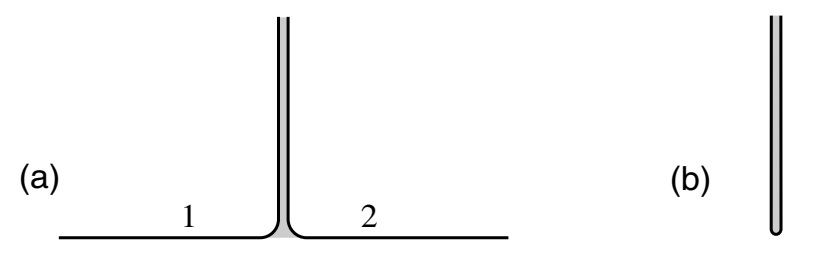
\includegraphics[width=0.8\textwidth,natwidth=630,natheight=195.75]{Fig9.10.jpg}\\
		\caption{Fig. 9.10. (a) $\Psi_{1} * \Psi_{2}$, convoluting the right half of $\Psi_{1}$ with the left half of $\Psi_{2}$. One can think of this as defined by a path integral over the shaded region, whose width is then taken to zero. (b) $\int \Psi$, convoluting the right and left halves of $\Psi$.}\label{Fig9.10}
	\end{center}
\end{figure}

为了给出相互作用理论,给规范变换加上非线性项
\begin{equation}
	\delta \Psi=Q_{\mathrm{B}} \Lambda+g \Psi * \Lambda-g \Lambda * \Psi
\end{equation}
$*$ 乘积是结合的,通过一个围道讨论可以证明 $Q_{\mathrm{B}}$ 像一个导数那样作用
\begin{equation}
	Q_{\mathrm{B}}\left(\Psi_{1} * \Psi_{2}\right)=\left(Q_{\mathrm{B}} \Psi_{1}\right) * \Psi_{2}+\Psi_{1} *\left(Q_{\mathrm{B}} \Psi_{2}\right)
\end{equation}
从这些可以得出 (9.6.8) 是封闭的. 利用循环性质
\begin{equation}
	\int \Psi_{1} * \Psi_{2}=\int \Psi_{2} * \Psi_{1}
\end{equation}
我们可以写下不变作用量
\begin{equation}
	S=\frac{1}{2} \int \Psi * Q_{\mathrm{B}} \Psi+\frac{2 g}{3} \int \Psi * \Psi * \Psi
\end{equation}
将其写成CFT的形式通常是有用的,将 $\Psi$ 替换成与顶点算符 $\mathscr{V} \Psi$对应的半圆盘
\begin{equation}
	S=\frac{1}{2}\left\langle\mathscr{V}_{\Psi} Q_{\mathrm{B}} \cdot \mathscr{V}_{\Psi}\right\rangle_{D_{2}}+\frac{2 g}{3}\left\langle\mathscr{V}_{\Psi} \mathscr{V} \psi \mathscr{V}_{\Psi}\right\rangle_{D_{2}}
\end{equation}
顶点算符位置和共形坐标系并不像(9.6.12) 中标出的那样,而是如\ref{Fig9.11}所示,一个 $z^{2 / 3}$ 映射将三顶角半圆盘调整成圆盘. 这个作用量通过了一个非常重要的检验. 仅对总 $Q^{g}=3$的插入,圆盘上的路径积分才是非零的. 物理态的顶点算符都有鬼数1,所以(9.6.12) 的两项都是非零的. 既然 (9.6.11) 是不变的,我们预期对于规范场,它退化至non-Abelian Yang-Mills作用量,而现实也的确如此.\\
Siegel规范是$b_{0} \Psi=0 $ . 在动能作用量中, $Q_{\mathrm{B}}$ 只有 $c_{0} L_{0}$ 项幸存下来. 既然在分量 $L_{0} \propto p^{2}+m^{2}$, 这类似于熟悉的电动力学协变规范. 传播子
\begin{equation}
	\int_{0}^{\infty} d t \exp \left(-t L_{0}\right)=L_{0}^{-1}
\end{equation}
就是对任意长度的带子积分. 顶点就是图\ref{Fig9.11}b中将楔子移去,将三个带子的末端插入了一个 ' $Y$' 中.

\begin{figure}
	\begin{center}
		%width=0.8\textwidth,bb=0 0 904 352
		%1px=0.75pt
		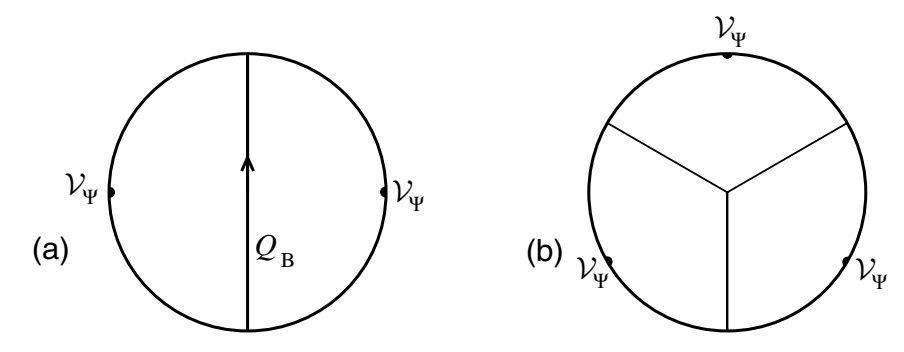
\includegraphics[width=0.8\textwidth,natwidth=678,natheight=264]{Fig9.11.jpg}\\
		\caption{Fig. 9.11. CFT representation of the string field action: (a) the kinetic term; (b) the interaction. A $z^{2 / 3}$ conformal transformation is used to turn the usual semi-circle around each vertex operator into a wedge.}\label{Fig9.11}
	\end{center}
\end{figure}

已经证明,这等价于用Riemann面求和描述的开弦理论,特别地,这个求和中包含对模空间的完整单覆盖. 另一方面,这是不惊奇的:弦场论有时空规范不变性 (9.6.8), 这使得空态会从S矩阵中退耦. 我们已经论证了空态的退耦决定了弦振幅的形式,这其中包括了模空间单覆盖的要求(否则全导数项会给出空态耦合). 另一方面,模空间十分复杂,只有少数几个有显式描述. 由这个弦场论产生的模空间,按Feynman图的求和且每张图写成对带长度的积分,在经由弦场论发现之前,数学家只稍微提前点发现它们.
\footnote{Another physically motivated description of moduli space comes from the light-cone gauge, where the moduli are the interaction times and the momenta $p^{+}$ of the intermediate states, and also a twist angle for each intermediate closed string.}

我们来指出这个场论的一个奇怪特征. 我们已经声明了弦场论覆盖了整个模空间,但是我们从圆环知道,即使不存在显式的闭弦场,这个模空间会包含产生闭弦极点的极限. 闭弦极点来自于带长趋于零的极限而非趋于无穷的极限. 
\footnote{For this reason, this form of string field theory would not be suitable for our purposes of the previous section. We would need to add stubs to the vertex to eliminate the unexpected divergences, and then to add in closed string propagators and vertices to cover the omitted region of moduli space.}
精确的陈述是开弦场路径积分生成了开弦论加上闭弦论的振幅(除了根本没有边界的曲面,这样的曲面开弦无法耦合). 在这一方面,以一种不精确的含义,闭弦就像是开弦的束缚态.\\
对于只有闭弦的理论,我们可以用闭弦场重复上面的步骤. 但这将会有点复杂. 对于自由作用量(9.6.3) ,鬼数就已经无法胜任了:为了使得物理态之间的矩阵元不为零,我们需要一个额外的 $c$鬼. 这里有一个补救,它要求弦场 $\Psi$ 和规范变换 $\Lambda$ 被 $b_{0}-\tilde{b}_{0}$ 和 $L_{0}-\tilde{L}_{0} $湮灭. 那么,作用量
\begin{equation}
	S_{0}^{\prime}=\frac{1}{2}\left\langle\left\langle\Psi\left|\left(c_{0}-\tilde{c}_{0}\right) Q_{\mathrm{B}}\right| \Psi\right\rangle\right.
\end{equation}
就在 $\delta \Psi=Q_{\mathrm{B}} \Lambda $下不变. 去往相互作用理论不再存在类似于 $*$的可结合乘积,相应地没有模空间的单覆盖. 就像上节那样,为了覆盖模空间,我们需要加入高阶顶角$\mathscr{V}_{g, n}$, 这样的顶角有更高层次的场以及内柄. 类似于开弦作用量,相应的作用量可以利用所谓的Batalin-Vilkovisky形式理论从对称性原理中得出. 然后,规范固定给出了上一节描述的微扰论.\\
从时空规范对称性导出弦论的推导是极其优雅的,尤其对于开弦,在开弦场论中引入闭弦是十分吸引人的. 然而,尚未知晓弦场论是否是超出微扰论的有用工具. 在当代基于时空超对称性的非微扰发展中,弦场论并没有起到什么作用,而这样的发展将在第14章进行讨论. 相当有可能的是,对于弦论的非微扰构建,弦,或者弦场,不简单地就是它的正确自由度.

\section{高阶行为}%{9.7 Large order behavior}
弦微扰论的高阶行为有一个有趣的结果. 我们先从场论出发. 考察积分
\begin{equation}
	\int_{-\infty}^{\infty} d y \exp \left[-\frac{y^{2}}{2 !}-\lambda \frac{y^{3}}{3 !}\right]=\lambda^{-1} \int_{-\infty}^{\infty} d z \exp \left[-\frac{1}{\lambda^{2}}\left(\frac{z^{2}}{2 !}+\frac{z^{3}}{3 !}\right)\right]
\end{equation}
其中$z=y \lambda $. 这个积分在 $\lambda \neq 0$时发散,但我们暂且忽视它,用 $\lambda$的形式幂级数计算它
\begin{equation}
	\sum_{n=0}^{\infty} \frac{(-\lambda)^{n}}{6^{n} n !} \int_{-\infty}^{\infty} d y y^{3 n} \exp \left(-y^{2} / 2\right)=(2 \pi)^{1 / 2} \sum_{k=0}^{\infty} \lambda^{2 k} C_{2 k}
\end{equation}
其中
\begin{equation}
	C_{2 k}=\frac{2^{k} \Gamma(3 k+1 / 2)}{\pi^{1 / 2} 3^{2 k}(2 k) !}
\end{equation}
这个积分是标量场论的零维极限,这个标量场论中有一个质量项和立方耦合. $\lambda$的展开可以表示成 Feynman图,图的传播子是1,而顶角是 $-\lambda$. 这样常数 $C_{2 k}$ 就计数了有$2 k$ 个立方顶角的真空图的总数. 等价地,是 $k+1$ 个圈的真空图总数,而每个图被赋予了合适的对称因子. 例如,读者可以验证有两个顶角的真空图有两个,而其对称群的阶分别是8和12,而 $C_{2}=\frac{5}{24}=\frac{1}{8}+\frac{1}{12}$. 为了得到高阶行为,我们使用Stirling近似 $n ! \approx n^{n+1 / 2} e^{-n}$,那么
\begin{equation}
	C_{2 k} \approx k^{k} \approx k !
\end{equation}
其中近似是在相差一个形式为$k^{a}$和$b^{k}$的因子下成立的.\\
我们还可以引入四次项 $\lambda^{2} y^{4} / 4 !$, 这使得积分收敛.  $\lambda$ 的幂次通过要求 $z$的作用量中的所有项均正比于 $\lambda^{-2} $ 决定;或者等价地,所有 $k+1$ 圈真空图被赋予权重$\lambda^{2 k} $ ,这个额外项并不会对结果有实质性的改变,估计(9.7.4)在一定的精度下依旧是成立的.\\
当考察场论时,传播子和顶角变得更加复杂. 然而,高阶处的主导行为往往来自于对图的计数————除非存在不寻常的IR行为或UV行为,传播子和顶角通常贡献阶为 $b^{k}$的因子. 级数的形式如下
\begin{equation}
	\sum_{k=0}^{\infty} \lambda^{2 k} k ! f_{2 k}
\end{equation}
其中 $f_{2 k} \approx k^{a} b^{k}$,它的变化要比 $k !$慢得多. 除非 $f_{2 k}$ 中有出乎意料的抵消,这会发散. 对于很小的 $\lambda$,这会暂时变得很小,随后像$k !$ 那样增长. 求和中最小项的阶是
\begin{equation}
	\exp \left[-O\left(1 / \lambda^{2}\right)\right]
\end{equation}
这是微扰论精度是一个渐近展开的特征. 诚然,像瞬子或者动力学对称性破缺的效应,它们在微扰论的所有阶都为零. 这样的效应一般是这一阶的. 例如,级数 $(9.7 .2)$的高阶行为与$z=-2$处的瞬子(稳定点)相关. 瞬子的作用量是 $2 / 3 \lambda^{2}$.\\
在弦理论中,模空间的Feynman图使得我们完全有可能构建出相同的约束. 对于形式为 (9.7.5) 的级数,若 $f_{2 k}$ 正定且有下界 $b^{k}$,这已经被显式地证明了. 因此,这个级数是发散的,甚至不是 Borel 可求和的. Borel求和将级数(9.7.5) 重写为对另一个更收敛级数的Laplace变换
\begin{equation}
	\int_{0}^{\infty} d t \exp (-t) \sum_{k=0}^{\infty}\left(t \lambda^{2}\right)^{k} f_{2 k}
\end{equation}
然而,$f_{2 k}$ 的正定性暗示了这个新的求和即使收敛但在正实轴上有极点,所以这个积分是病态的. 因此,我们预期弦理论会有一个有趣的非微扰现象. 这并不奇怪,因为在低能极限下,它们退化至非平庸的场论.\\
估计 (9.7.4) 对于闭弦理论是个下界,这可以通过只保留树图立方顶角$\mathscr{V}_{0,3} $ 获得. 由于闭弦顶角会从所有亏格的Riemann面处得到修正,我们会好奇是否微扰论会增长得更快. 看到它确实如此的一个方法是回忆起开弦场论包含所有开弦Riemann面,以及至少有一个边界的闭弦Riemann面. 我们来考察只有一个边界的曲面,所在的区域为边界收缩至一个点. 开弦模空间的极限等于有一个顶点算符的闭曲面的模空间. 可以证明这个区域并不比整个开弦模空间小多少. 所以相同的估计依旧成立. 微扰级数趋于
\begin{equation}
	\sum_{k=0}^{\infty} g_{0}^{2 k} O(k !)=\sum_{k=0}^{\infty} g_{\mathrm{c}}^{k} O(k !)
\end{equation}
亏格为 $g$ 的项正比于 $g_{\mathrm{c}}^{2 g}$, 它有一个阶为 $(2 g) ! $的系数.  这要大于场论的$g !$特征,这样的特征同时是只从 $\mathscr{V}_{0,3}$ 获得的下界. 显然,高阶振幅的最大部分被包含在顶角 $\mathscr{V}_{g, n}$ 中并来自于模空间的内部,可以预期非微扰效应的量级是
\begin{equation}
	\exp \left[-O\left(1 / g_{\mathrm{c}}\right)\right]
\end{equation}
它在弱耦合处远大于场论特征$\exp \left[-O\left(1 / g_{\mathrm{c}}^{2}\right)\right]$ . 高阶行为是在9.9节将要讨论的一些简化模型中首先观察到的. 我们将会在第13章看到,至少是在某些超弦理论中,这些效应已知是与D膜相关的.


\section{高能和高温}%{9.8 High energy and high temperature}

为了对弦动力学有更好的理解,我们可以看一下它在不同极限下的行为. 在这一节,我们考察弦论的各种高能极限.
\subsection*{\centerline{Hard scattering(硬散射)}}
再一次考察硬散射行为,这样的行为是通过对 Veneziano振幅和 Virasoro-Shapiro 振幅做 Stirling近似获得的. 回到积分形式(6.6.5),
\begin{equation}
	\frac{8 \pi i g_{\mathrm{c}}^{2}}{\alpha^{\prime}}(2 \pi)^{26} \delta^{26}\left(\sum_{i} k_{i}\right) \int_{\mathbf{C}} d^{2} z_{4}\left|z_{4}\right|^{-\alpha^{\prime} u / 2-4}\left|1-z_{4}\right|^{-\alpha^{\prime} t / 2-4}
\end{equation}
在$t / s$保持固定, $s \rightarrow \infty$ 的硬散射区域,指数很大,积分由指数的稳定点主导. 
\footnote{As usual, the integral diverges at $z_{4} \rightarrow \infty$ and is defined by analytic continuation. The saddle point approximation can be justified for the continuation. }
当 $s, t, u \gg 1$时,鞍点是
\begin{equation}
	\frac{\partial}{\partial z_{4}}\left(u \ln \left|z_{4}\right|^{2}+t \ln \left|1-z_{4}\right|^{2}\right)=\frac{u}{z_{4}}+\frac{t}{z_{4}-1}=0
\end{equation}
回忆 $s+t+u=O(1) $,其解是 $z_{4}=-u / s $ . 那么鞍点近似给出振幅
\begin{equation}
	S \approx \exp \left[-\alpha^{\prime}(s \ln s+t \ln t+u \ln u) / 2\right]
\end{equation}
同(6.6.13)给出的一样.\\
让我们后退一步,以$z_{4}$ 的积分回到对 $X^{\mu} $的路径积分. 它由鞍点主导
\begin{equation}
	X_{\mathrm{cl}}^{\mu}(\sigma)=i \sum_{i} k_{i}^{\mu} G^{\prime}\left(\sigma, \sigma_{i}\right)
\end{equation}
其中$\sigma_{i}$ 是顶点算符位置. 回忆Green函数正比于$\alpha^{\prime}$. 在高能,散射区域的尺寸随着能量线性增长, $\delta X \approx \alpha^{\prime} k$. 在场论中,高能硬散射探测小距离,通过不确定原理 $\delta X \approx 1 / k$ 在弦论中,当超过弦标度之后就不是这样的情况. 在弦微扰论中表现为不可能探测小于这个标度的距离,这给出这样的概念,它是时空中的极限距离. 紧致化上的有效下界 $R \approx \alpha^{1 / 2}$ 也支持这一点. 然而,我们会在第13章看到,非微扰弦论中的一些最新发展揭示了更低距离标度的存在.\\
在弦圈展开的一般阶,振幅中的主导项是
\begin{equation}
	\exp \left[-\sum_{i<j} k_{i} \cdot k_{j} G^{\prime}\left(\sigma_{i}, \sigma_{j}\right)\right]
\end{equation}
我们需要找到这个指数的鞍点,即针对顶点算符的位置. 又要针对Riemann面的模. 这很像一个静电学问题:指数是 $n$ 个带电 $k_{i}^{\mu}$ 粒子在Riemann面上的能量,其中 $\mu$ 标记 $d$ 个不同的静电场,而$\mu=0$ 在能量上有相反的符号. 背景电荷密度由于动量守恒为零,由于 $k_{i}^{2}$在壳且很小,所以重整化自能可以忽略. 相当显著的是,在每一个亏格 都会发现疑似鞍点. 考察Riemann面
\begin{equation}
	z_{2}^{N}=\frac{\left(z_{1}-a_{1}\right)\left(z_{1}-a_{2}\right)}{\left(z_{1}-a_{3}\right)\left(z_{1}-a_{4}\right)}
\end{equation}
同超几何曲线 (9.2.9)一样,它是$S_{2} \times S_{2}$的子空间. 它可以视为 $N$面在割线处粘在一起,并有亏格 $N-1$. 对于四点振幅,如果电荷处在割线 $a_{i}$处,振幅相对它们的位置是稳定的————曲面在这些点是“垂直”的,$\partial z_{2} / \partial z_{1}=\infty$, 而对称性 $z_{2} \rightarrow \exp (2 \pi i / N) z_{2}$ 要求梯度的垂直分量为零.
相对于位置$a_{i}$它还有些极端,但这是很容易的:电场与球面上电荷在$z=a_{i}$处的电场相同,不同之处在于它分成了$N$ sheets. 因此,能量是球面上的 $N \cdot N^{-2}=N^{-1}$ ,其中的三个位置可以被Möbius变换固定到 $0,1, \infty$, 而第四个由球面上的条件$(9.8 .2)$给出. 因此在亏格 $g$
\begin{equation}
	S_{g} \approx \exp \left[-\alpha^{\prime}(s \ln s+t \ln t+u \ln u) / 2(g+1)\right]
\end{equation}
经过额外的努力,可以引入鞍点附近的Gaussian涨落,这决定了$S_{g} $的系数. 对于$N$ -sheeted 鞍点, $X_{\mathrm{cl}}^{\mu}$ 只需除以 $N=g+1$即可.\\
这里有一个方法可以检验这个结果确实是合理的. 在 $-t / s \ll 1$ 的小角区域,它变成
\begin{equation}
	\exp \left[\alpha^{\prime} t \ln s / 2(g+1)\right]
\end{equation}
现在, $t^{1 / 2}$ 是从入射粒子1到末态粒子3的总转移动量. 在小角区域,亏格为g的散射过程看上去可以分解成 $g+1$ 个连续散射. 每个散射有相同的质心 $s$, 而$t_{i}$ 要满足总转移动量为 $t^{1 / 2}$的约束. 单个散射趋于 $\exp \left(\alpha^{\prime} t_{i} \ln s / 2\right)$. 那么很容易验证取动量传递相等是最有效的, 即$t_{i}^{1 / 2}=t^{1 / 2} /(g+1)$, 这给出振幅之积的结果$(9.8 .8)$ . 这不同于粒子散射,在那里最有效的是将动量传递给几个硬散射.\\
对于激发弦态,顶点算符的指数行为与快子相同. 那么主导行为为同一个鞍点.  $X_{\mathrm{cl}}^{\mu}$被代入了顶点算符之中. 既然除了一个 $g+1$因子,所有态且所有阶的主导鞍点均相同,在不同态的散射之间存在一个线性关系,它对于所有亏格都成立,因而对于精确振幅也很可能是成立的. 在量子场论中,高能散射通常会揭示在低能不明显的对称性. 大家广泛认同这里所发现的关系属于同一类.\\
现在仍然不清楚级数 (9.8.7)的和在什么情况下是有意义的. 对比这一节与上一节的结果是有意义的. 在这两种情况,产生有趣物理结果是模空间内部(与之对照的是,场论行为是在边界发生的). 然而高阶行为来自于整个模空间,特别地,这个行为由模空间的大体积主导 . 而固定亏格处的高能行为由单个点主导.

\subsection*{\centerline{Regge scattering(Regge散射)}}
对Regge极限的分析也可推广至更高阶. 我们不会做这件事,但是会对树图Regge物理发展一个有趣的解释. 对于大多数物理学家,Regge散射没有硬散射那么熟悉. 它是高增速系统的一个温和探针. 当一个系统被增速后,时间伸缩子会减慢它的内部过程. 那么当一个高能系统趋于高能时,我们可以期望看到更多虚自由度.\\
我们来考察单个弦的量子涨落. 它的平方根意味着基态的尺度. 模展开给出
\begin{equation}
	\begin{aligned}
		\left\langle 0\left|\left[X^{1}(\sigma)-x^{1}\right]^{2}\right| 0\right\rangle &=\sum_{n=1}^{\infty} \frac{\alpha^{\prime}}{2 n^{2}}\left\langle 0\left|\left(\alpha_{n} \alpha_{-n}+\tilde{\alpha}_{n} \tilde{\alpha}_{-n}\right)\right| 0\right\rangle \\
		&=\alpha^{\prime} \sum_{n=1}^{\infty} \frac{1}{n}
	\end{aligned}
\end{equation}
这是发散的,但是没有直接的物理意义. 在时间标度 $\delta \tau$上的测量仅对于频率小于 $\delta \tau^{-1}$的模是敏感的,而又有 $n \alpha^{\prime-1 / 2}<\delta \tau^{-1}$. 对数发散变成 $\alpha^{\prime} \ln \left(\alpha^{1 / 2} / \delta \tau\right)$, 而尺寸是它的平方根.\\
有效尺寸的增长在$t$很小的 Regge 振幅 (6.6.12) 中是可以直接观察的
\begin{equation}
	s^{2+\alpha^{\prime} t / 2} \frac{\Gamma\left(-\alpha^{\prime} t / 4-1\right)}{\Gamma\left(\alpha^{\prime} t / 4+2\right)} \sim \frac{s^{2}}{t} \exp \left[-\frac{q^{2} \alpha^{\prime}}{2} \ln \left(\alpha^{\prime} s\right)\right]
\end{equation}
其中$q^{2}=-t$是动量转移. 这是一个被形状因子修正的引力振幅 $s^{2} / t$ ,形状因子的Fourier变换对应于一个尺寸为 $\left(\alpha^{\prime} \ln \alpha^{\prime} s\right)^{1 / 2}$的物体. 从一个弦的视角来看,另外一个有阶为$\alpha^{\prime} s$的增速,所以它的内部过程的时间分辨反比于它,与这个尺寸的早先估计一致.\\
对数的平方根是一个增长很慢的函数,一般没有什么意义,但需要提醒的是,这个行为对于黑洞附近的弦非常重要. 在第14章我们会以一个不同的视角回顾这一点,弦的概念在增速很高时揭示出了它们的真实特性.

\subsection*{\centerline{High temperature(高温)}}
弦行为变得有趣的另一个极限是高温. 从配分函数在高权重$h$的一般行为(7.2.30) ,以及关系 $m^{2}=4(h-1) / \alpha^{\prime}$, 弦态的密度 $n(m)$ 满足
\begin{equation}
	\int_{0}^{\infty} d m n(m) \exp \left(-\alpha^{\prime} \pi m^{2} \ell\right) \approx \exp (4 \pi / \ell)
\end{equation}
这暗示了 $n(m) \approx \exp \left(4 \pi m \alpha^{\prime 1 / 2}\right)$. 那么单个弦的热配分函数就是
\begin{equation}
	\int_{0}^{\infty} d m \exp \left(4 \pi m \alpha^{\prime 1 / 2}\right) \exp (-m / T)
\end{equation}
因为态密度指数增长,当温度高于一定值时,配分函数 (9.8.12) 会发散,这样的温度称为 Hagedorn温度
\begin{equation}
	T_{\mathrm{H}}=\frac{1}{4 \pi \alpha^{\prime 1 / 2}}
\end{equation}
可以对Hagedorn发散有如下理解. 长弦的能量正比于它的长度,它的熵也是这样,是广延量. 在低温,能量主导;在高温,熵主导,并且倾向于产生各种长度的弦. 在这种弦的系综中,密度会变大,并且相互作用在相变点附近会变得重要. \\
这一发散表明有一相变. 事实也的确如此. 在高激发强子的态密度有一个类似的增长,并且从低温强子相到高温夸克-胶子等离子体相有一个相变. 一个有趣的问题是,Hagedorn发散是否表明在基本弦中有类似夸克-胶子结构,但这个问题没有明确的答案. \\
为了总结,我们来更加细致地讨论自由弦的配分函数. 在$d$维中,质量为$m$的实标量场的自由能密度是
\begin{equation}
	\begin{aligned}
		F\left(T, m^{2}\right) &=T \int \frac{d^{d-1} \mathbf{k}}{(2 \pi)^{d-1}} \ln \left[1-\exp \left(-\omega_{k} / T\right)\right] \\
		&=-\int_{0}^{\infty} \frac{d t}{t}(2 \pi t)^{-d / 2} \sum_{r=1}^{\infty} \exp \left(-\frac{m^{2} t}{2}-\frac{r^{2}}{2 T^{2} t}\right)
	\end{aligned}
\end{equation}
在第二个形式中,已经可以对弦谱求和. 沿用真空振幅(7.3.12) 和 (7.3.6)的推导,26平坦维中自由能密度是
\begin{equation}
	F(T)=-\int_{R} \frac{d \tau d \bar{\tau}}{2 \tau_{2}}\left(4 \pi^{2} \alpha^{\prime} \tau_{2}\right)^{-13}|\eta(\tau)|^{-48} \sum_{r=1}^{\infty} \exp \left(-\frac{r^{2}}{4 \pi T^{2} \alpha^{\prime} \tau_{2}}\right)
\end{equation}
这个积分跑遍整个区域
\begin{equation}
	R: \quad \tau_{1} \leq \frac{1}{2}, \quad\left|\tau_{2}\right|>0
\end{equation}
在 $\tau_{2} \rightarrow 0 $时有一个可能的发散;当 $\tau$ 的实部为零时,被积函数为极大值,所以令 $\tau=i \tau_{2}$. 从模变换(7.2.44),  eta函数在这一极限下的渐近行为是
\begin{equation}
	\begin{aligned}
		\eta\left(i \tau_{2}\right) &=\eta\left(i / \tau_{2}\right) \tau_{2}^{-1 / 2} \\
		& \approx \exp \left(-\pi / 12 \tau_{2}\right) \text { as } \tau_{2} \rightarrow 0
	\end{aligned}
\end{equation}
因此, $\tau$ 的积分在 $T<T_{\mathrm{H}}$ 收敛,在 $T>T_{\mathrm{H}}$发散.\\
在场论中,配分函数由 Euclidean 路径积分给出,其时间有周期 $1 / T$. 在弦论中发生了同样的事情. $T$ 对偶理应将高温行为与低温行为关联起来. 事实上,Hagedorn 温度是自对偶值的一半. 定义
\begin{equation}
	\tilde{F}(T)=F(T)+\rho_{0}
\end{equation}
自由能的热部分(9.8.15) 加上真空部分 (7.3.6). 这个路径积分的对数是 $-\tilde{F}(T) / T$, 所以 $T$ 对偶暗示了
\begin{equation}
	\frac{1}{T} \tilde{F}(T)=\frac{T}{4 T_{\mathrm{H}}^{2}} \tilde{F}\left(4 T_{\mathrm{H}}^{2} / T\right)
\end{equation}
这将Hagedorn温度以下的与Hagedorn温度以上的配分函数关联起来. $T>T_{\mathrm{H}}$时Hagedorn发散是低温理论中快子发散的一个反映,但是在超弦中有一个类似的形式结果,而超弦中是没有快子发散的. 如果我们严格地取这个关系,在$T \rightarrow \infty $时,我们获得
\begin{equation}
	\tilde{F}(T) \rightarrow \frac{T^{2}}{4 T_{\mathrm{H}}^{2}} \rho_{0}
\end{equation}
如果这衡量了高温自由度数,那么这是相当少的.  $d$ 维时空中的单个量子场拥有阶为 $T^{d}$的自由能. 所以,弦理论的高温极限看起来就像是两个时空维中的场论. 这完全不像Hagedorn相变以下指数增长的频谱,可能是揭示相变性质的一个线索.

\section{低维和非临界弦}%{9.9 Low dimensions and noncritical strings}
场论通常会随着时空维数的减少而简化,而这些低维理论是理解动力学的有用模型. 我们可以尝试在弦论中做同样的事情. 但弦论要求临界维数. 我们可以紧致化,但这不会减少自由度的个数. 弦仍然在紧致维中振荡. 然而,我们遇到过一个相容的背景. 在这个背景场中,弦实际上在更低维度中运动. 这是线性伸缩子背景(3.7.18)
\begin{subequations}
\begin{equation}
		G_{\mu v}(x) =\eta_{\mu v}, \quad B_{\mu v}(x)=0, \quad \Phi(x)=V_{\mu} x^{\mu} 
\end{equation}
\begin{equation}		
		V_{\mu} =\delta_{\mu}^{1}\left(\frac{26-D}{6 \alpha^{\prime}}\right)^{1 / 2}
\end{equation}
\end{subequations}
当$D<26$ 时,伸缩子梯度是类空的,我们已经将其取到1方向上.\\
有效弦耦合 $e^{\Phi}$ 是 $x^{1}$的函数,在大 $x^{1}$ 处发散. 这使得很难使用弦微扰论,但幸运的是存在另一个稍微不同的背景,在这个背景下微扰论是好的. 将背景(9.9.1)代入快子作用量 (6.6.16)给出线性快子场方程
\begin{equation}
	-\partial^{\mu} \partial_{\mu} T(x)+2 V^{\mu} \partial_{\mu} T(x)-\frac{4}{\alpha^{\prime}} T(x)=0
\end{equation}
这是能动张量为线性伸缩子能动张量(2.5.1)时,指数顶点算符是Weyl不变的条件. 它的解是
\begin{equation}
	T(x)=\exp (q \cdot x), \quad(q-V)^{2}=\frac{2-D}{6 \alpha^{\prime}}
\end{equation}
如果我们寻求伸缩子这种只依赖于 $x^{1}$的解,那么
\begin{equation}
	q_{1}=\alpha_{\pm}=\left(\frac{26-D}{6 \alpha^{\prime}}\right)^{1 / 2} \pm\left(\frac{2-D}{6 \alpha^{\prime}}\right)^{1 / 2}
\end{equation}
当 $D>2$时,这是复数,所以快子振荡. 但当 $D \leq 2$时,会得到实指数 (在临界值 $D=2$ 乘以线性函数). 当然,快子场方程有非线性修正. 可以证明,除了一些相当微妙的原因,只有$\alpha_{-}$ 会给出不奇异背景外,这不会影响背景场的定性形式.\\
对$D \leq 2$ ,对于弦基态而言,“快子”实际上不是一个恰当的术语,这是因为场是稳定的. 另外,当$D \leq 2$时,实指数 $T(x)=T_{0} \exp \left(\alpha_{-} x^{1}\right)$ 阻止了向大 $x^{1}$ 区域的传播,这一区域的耦合是发散的. 为了看到这点,考察世界面作用量
\begin{equation}
	S_{\sigma}=\frac{1}{4 \pi \alpha^{\prime}} \int_{M} d^{2} \sigma g^{1 / 2}\left[g^{a b} \eta_{\mu v} \partial_{a} X^{\mu} \partial_{b} X^{v}+\alpha^{\prime} R V_{1} X^{1}+T_{0} \exp \left(\alpha_{-} X^{1}\right)\right]
\end{equation}
当$x^{1}$很大时,指数快子会主导线性伸缩子,而路径积分被压低了. 这对应于弦的由快子背景引起的有效势. 物理上,拥有渐近区域$x^{1} \rightarrow-\infty$, 在这一区域耦合趋于零. 向正 $x^{1}$ 传播的弦与其他弦相互作用,并被有效势反弹回到渐近区域. 最大有效耦合被势的能量与强度$T_{0}$ 设定. 如图\ref{Fig9.12},这一图景有些新奇,但就寻找可解模型的方面而言,它是值得追求的. 一个相当类似的物理的模型————静态模型,在揭开量子场论特性方面扮演了重要角色.

\begin{figure}
	\begin{center}
		%width=0.8\textwidth,bb=0 0 648 567
		%1px=0.75pt
		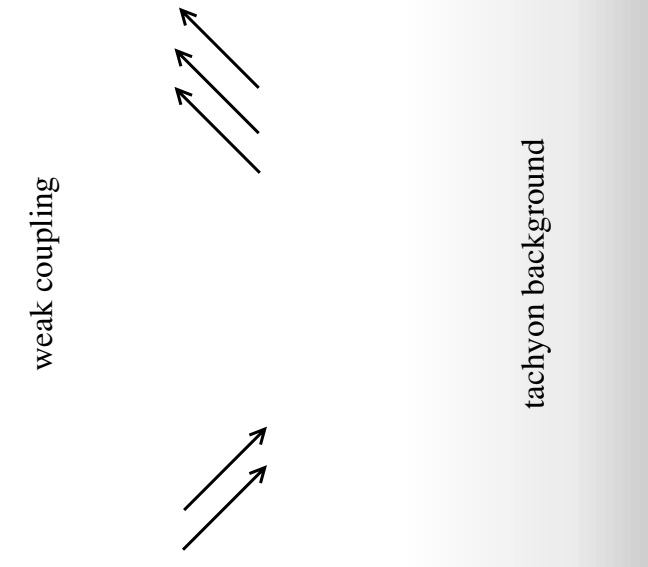
\includegraphics[width=0.5\textwidth,natwidth=486,natheight=425.25]{Fig9.12.jpg}\\
		\caption{Fig. 9.12. Spacetime with dilaton and tachyon backgrounds. The interaction strength grows toward the right but is cut off by an effective potential from the tachyon background.}\label{Fig9.12}
	\end{center}
\end{figure}

当$D>2$ 时,尽管已经论证了快子背景的作用像个势垒,但它的物理效应并不非常清晰. 然而,将注意力集中在 $D \leq 2$ 上有另一个原因,即这些理论实际上是可解的. 我们先来观察,当我们量子化弦时,规范对称性会带走两族振子. 这使得 $D \leq 2$ 时什么也不会被剩下————只有质心运动,一个标量. 
\footnote{ At special momenta one finds additional physical states. These can be interpreted as unbroken symmetries of string field theory, and likely play a role in the solvability of the theory. }
然而,直接解这个弦论是相当困难的. 首先,必须要计算作用量为(9.9.5)的世界面路径积分. 由于指数快子场,这不再是自由理论. 它被称为 Liouville场论. 它是经典可积的,再经过一些努力后,可以定出一些量子振幅. 然而,为了解出弦理论,我们需要在Riemann面模空间的每个亏格上积这个结果,我们已经看到这是一个紧致空间. 相当显著的是,通过相当不同的方法,直至所有阶的振幅已被确定下来. 为了描述这个方法,我们必须先引入另一个概念.

\subsection*{\centerline{Noncritical strings(非临界弦)}}
考察统计力学系统,它由对 $d$ 维Euclidean空间中的二维曲面求和定义. 我们同时假定曲面有一些可以解释为长度测度的内部自由度. 描述这个系统的自然场是嵌入$X^{\mu}(\sigma)$ 与度规 $g_{a b}(\sigma) $ . 然而,没有什么理由将长度扔出这个问题————即,理论不一定是Weyl不变的. 因而,这被称为非临界弦. 这个系统的最低维作用量是有额外世界面常数项的 Polyakov作用量,这样的项在临界弦中会被Weyl不变性所禁止
\begin{equation}
	S=\frac{1}{4 \pi \alpha^{\prime}} \int_{M} d^{2} \sigma g^{1 / 2}\left(g^{a b} \partial_{a} X^{\mu} \partial_{b} X_{\mu}+\mu\right)
\end{equation}
没有Weyl不变性,我们可以用diff不变性部分地确定度规,但会剩余一个自由度
\begin{equation}
	g_{a b}(\sigma)=\exp (2 \phi(\sigma)) \hat{g}_{a b}(\sigma)
\end{equation}
其中 $\hat{g}_{a b}$是规范选择,而度规的标度$\phi$ 仍然要路径积分. 这一个规范固定的 Faddeev-Popov行列式与(3.4.19)相同,  Weyl固定对后者的贡献是平庸的. 代入度规 (9.9.7), 曲率是
\begin{equation}
	g^{1 / 2} R=\hat{g}^{1 / 2}\left(\hat{R}-2 \hat{\nabla}^{2} \phi\right)
\end{equation}
扔掉场无关项,这个作用量加上Faddeev-Popov行列式变成
\begin{equation}
	S=\frac{1}{4 \pi \alpha^{\prime}} \int_{M} d^{2} \sigma \hat{g}^{1 / 2}\left[\hat{g}^{a b} \partial_{a} X^{\mu} \partial_{b} X_{\mu}+\mu \exp 2 \phi+\frac{13 \alpha^{\prime}}{3}\left(\hat{g}^{a b} \partial_{a} \phi \partial_{b} \phi+\hat{R} \phi\right)\right]
\end{equation}
注意到, Faddeev-Popov行列式为 $\phi$提供了动能项. 与伸缩子-快子作用量 (9.9.5) 相比,我们看到一个显著的相似之处. 如果我们令 $d=D-1$,并将新的场 $\phi$ 解释成 $x^{1}$, 并且在作用量(9.9.5)中重命名 $g_{a b} \rightarrow \hat{g}_{a b}$ ,那么相同的项都会出现. 一些系数会有些不同————不存在$\phi$的重标度使得它们均一致————但事实上,我们声称是同一个场论. 关键在于,定义临界弦路径积分(9.9.5) 时是将 $\hat{g}_{a b}$ 用作度规,而非临界弦(9.9.9)用的是 $\exp (2 \phi) \hat{g}_{a b} $. 
对测度的Weyl变换的一个小心处理,可以将一个转换成另一个. 注意到,只有整个度规(9.9.7) 出现在临界弦的定义中,这使得理解这点很容易. 这个事实,使得在变换
\begin{subequations}
\begin{equation}
		\hat{g}_{a b}(\sigma)  \rightarrow \exp (2 \omega(\sigma)) \hat{g}_{a b}(\sigma) 
\end{equation}
\begin{equation}		
		\phi(\sigma)  \rightarrow \phi(\sigma)-\omega(\sigma)
\end{equation}
\end{subequations}
因此非临界弦获得了Weyl不变性,而这足以固定自由参量 $\mu$以外的各种系数.\\
Weyl不变的理论和非Weyl不变的理论可以等价,这看起来很奇怪. 关键在于,在场论中,如果我们同时增加仅用来固定规范的场,我们总可以增添额外的“假”规范对称性. 一个规范对称性毕竟只是冗余的描述,而我们总可以采用更冗余的描述. 对于对称性 (9.9.10) ,我们显然可以仅抵消场 $\phi$的Weyl对称性. 但对于一般的弦背景(例如平坦空间,那里嵌入坐标是Weyl不变的) ,这是不可能的,并且Weyl不变性是“真实的”.\\
在任何情况下,我们现在到达一个很微妙的境地,我们可以通过对三角化曲面的求和来近似非临界弦,两个点之间边的数目变成长度的测度. 这些三角化曲面类似于大Feynman图. 事实上我们可以找到一个量子系统————矩阵模型,使得这是一个图展开. 矩阵模型的场是$N \times N$ 矩阵. 取$N \rightarrow \infty$ 并调整其他耦合,(至少对于 $D \leq 2$ ) 存在由大光滑曲面主导的临界点. 所以我们恢复出了非临界弦. 更进一步,通过对角化矩阵(至少对于 $D \leq 2$ ) ,矩阵模型是可解的. 在最后我们会获得一个相当简单的系统 (非相互作用的费米子在本征值空间中运动),折回上面的步骤, 这使得弦振幅的计算可以到任意阶.\\
我们将细节留在参考文献中. 在任何情况下,当$D>2$时或者处于超对称理论中,还没发现它们是有用的. 然而,至少我们要提及从这些模型中所学到的重要一课. 微扰论中的$(2 g) !$ 行为,这最初是在显式矩阵模型中看到的,并由此论证它在所有弦论中成立. 在矩阵模型中,相应的 $\exp \left[O\left(-1 / g_{\mathrm{c}}\right)\right]$ 效应包括本征值空间中的费米子的隧道效应.这是否与高维弦论中的 $\exp \left[O\left(-1 / g_{\mathrm{c}}\right)\right]$ 效应有关联,现在仍然是不清楚的.
